%!TEX program = xelatex
%!TEX root = ../all_beamer.tex


%% Multilayer Networks – Beamer Presentation
%% Based on notes by Giorgio Gambosi, University of Rome "Tor Vergata"
%% Style modelled on ml-linclass-beamer.tex

%% !TEX root = all_beamer.tex
% ==============================================================================
% HEADER LATEX PER PRESENTAZIONI BEAMER
% Corso di Machine Learning - Giorgio Gambosi
% Università di Roma "Tor Vergata"
% ==============================================================================

% ------------------------------------------------------------------------------
% CLASSE DOCUMENTO E METADATI
% ------------------------------------------------------------------------------
\documentclass[aspectratio=169, 10pt]{beamer}

\subtitle{Course of Machine Learning}
\author{Giorgio Gambosi}
\institute[Tor Vergata]{Master's Degree in Computer Science\\University of Rome ``Tor Vergata''}
\date{A.Y. 2025--2026}

% ------------------------------------------------------------------------------
% PACCHETTI MATEMATICI
% ------------------------------------------------------------------------------
\usepackage{amsmath, amssymb, amsfonts, mathtools, amsthm}
\usepackage{bm}              % Simboli matematici in grassetto
\usepackage{upgreek}         % Lettere greche dritte
\usepackage{derivative}      % Gestione semplificata delle derivate

% ------------------------------------------------------------------------------
% PACCHETTI GRAFICI E VISUALIZZAZIONE
% ------------------------------------------------------------------------------
\usepackage{graphicx}        % Inclusione immagini
\usepackage{xcolor}          % Gestione colori
\usepackage{xkcdcolors}      % Colori aggiuntivi stile xkcd
\usepackage{microtype}       % Miglioramenti tipografici

% ------------------------------------------------------------------------------
% PACCHETTI PER TABELLE
% ------------------------------------------------------------------------------
\usepackage{booktabs}        % Tabelle professionali
\usepackage{array}           % Estensioni per tabelle
\usepackage{multirow}        % Celle multi-riga
\usepackage{multicol}        % Layout multi-colonna

% ------------------------------------------------------------------------------
% TIKZ E PGFPLOTS
% ------------------------------------------------------------------------------
\usepackage{tikz}
\usepackage{tikz-network}
\usepackage[customcolors]{hf-tikz}
\usepackage{pgfplots}
\pgfplotsset{compat=1.18}
\usepgfplotslibrary{fillbetween}

% Librerie TikZ
\usetikzlibrary{arrows, arrows.meta, decorations.pathmorphing, decorations.pathreplacing}
\usetikzlibrary{decorations.markings, snakes, positioning, backgrounds, fit, shadows}
\usetikzlibrary{automata, patterns, calc, intersections, through, shapes}
\usetikzlibrary{shapes.geometric, shapes.arrows, scopes, chains, matrix}

% ------------------------------------------------------------------------------
% ALTRI PACCHETTI
% ------------------------------------------------------------------------------
\usepackage[skins]{tcolorbox}  % Box colorati
\usepackage{subcaption}         % Sottocaption per figure
\usepackage{listings}           % Inclusione codice sorgente

% ------------------------------------------------------------------------------
% TEMA E STILE BEAMER
% ------------------------------------------------------------------------------
\usetheme{Madrid}
\usecolortheme{whale}
\useinnertheme{rounded}
\usefonttheme{professionalfonts}
\setbeamertemplate{navigation symbols}{}  % Rimuove simboli di navigazione

% ------------------------------------------------------------------------------
% DEFINIZIONE COLORI PERSONALIZZATI
% ------------------------------------------------------------------------------
% Colori principali del tema
\definecolor{MainBlue}{RGB}{31,56,100}      % Blu principale (header, titoli)
\definecolor{AccentBlue}{RGB}{70,130,180}   % Blu accento (blocchi)
\definecolor{AlertRed}{RGB}{160,30,30}      % Rosso per alert
\definecolor{ExGreen}{RGB}{30,120,60}       % Verde per esempi
\definecolor{BlockBg}{RGB}{220,232,246}     % Sfondo blocchi
\definecolor{torgray}{RGB}{220,225,235}     % Grigio Tor Vergata

% Colori alternativi (Tor Vergata style)
\definecolor{TvDark}{RGB}{30,50,80}         % Blu scuro header
\definecolor{TvMid}{RGB}{70,100,140}        % Blu medio blocchi
\definecolor{TvLight}{RGB}{210,220,235}     % Blu chiaro sfondi
\definecolor{TvAlert}{RGB}{160,30,30}       % Rosso alert
\definecolor{TvGreen}{RGB}{20,100,50}       % Verde esempi

% Colori supplementari
\definecolor{torred}{RGB}{153,0,0}
\definecolor{torcyan}{RGB}{0,112,192}
\definecolor{cerise}{HTML}{DA3A62}
\definecolor{teal}{HTML}{029386}
\definecolor{slateblue}{HTML}{5B5EA6}
\definecolor{orange}{HTML}{F97306}

% Colori per nodi TikZ
\definecolor{nodeblue}{RGB}{101,140,196}    % xkcd Faded Blue

% ------------------------------------------------------------------------------
% CONFIGURAZIONE COLORI BEAMER
% ------------------------------------------------------------------------------
\setbeamercolor{frametitle}{bg=MainBlue, fg=white}
\setbeamercolor{title}{bg=MainBlue, fg=white}
\setbeamercolor{structure}{fg=MainBlue}

% Blocchi standard
\setbeamercolor{block title}{bg=AccentBlue, fg=white}
\setbeamercolor{block body}{bg=BlockBg}

% Blocchi alert
\setbeamercolor{block title alerted}{bg=AlertRed, fg=white}
\setbeamercolor{block body alerted}{bg=red!8}

% Blocchi esempio
\setbeamercolor{block title example}{bg=ExGreen, fg=white}
\setbeamercolor{block body example}{bg=green!7}

% ------------------------------------------------------------------------------
% CONFIGURAZIONE FONT BEAMER
% ------------------------------------------------------------------------------
\setbeamerfont{frametitle}{size=\normalsize,series=\bfseries}
\setbeamerfont{block title}{size=\small,series=\bfseries}

% ------------------------------------------------------------------------------
% STILI TIKZ PERSONALIZZATI
% ------------------------------------------------------------------------------
\tikzset{
  >=latex,  % Frecce stile LaTeX di default
  % Nodi per reti neurali
  node/.style={thick,circle,draw=myblue,minimum size=22,inner sep=0.5,outer sep=0.6},
  node in/.style={node,green!20!black,draw=mygreen!30!black,fill=mygreen!25},
  node hidden/.style={node,blue!20!black,draw=myblue!30!black,fill=myblue!20},
  node convol/.style={node,orange!20!black,draw=myorange!30!black,fill=myorange!20},
  node out/.style={node,red!20!black,draw=myred!30!black,fill=myred!20},
  % Connessioni
  connect/.style={thick,mydarkblue},
  connect arrow/.style={-{Latex[length=4,width=3.5]},thick,mydarkblue,shorten <=0.5,shorten >=1},
  % Stili numerati per facile mappatura
  node 1/.style={node in},
  node 2/.style={node hidden},
  node 3/.style={node out}
}

% ------------------------------------------------------------------------------
% AMBIENTI TEOREMI
% ------------------------------------------------------------------------------
\setbeamertemplate{theorems}[numbered]
\newtheorem{mytheorem}{Theorem}
\newtheorem{mydefinition}{Definition}

% ------------------------------------------------------------------------------
% CONFIGURAZIONE LISTINGS (CODICE)
% ------------------------------------------------------------------------------
\lstset{
  language=Python,
  basicstyle=\ttfamily\tiny,
  keywordstyle=\color{MainBlue}\bfseries,
  commentstyle=\color{gray},
  frame=single,
  breaklines=true,
}

% ==============================================================================
% MACRO MATEMATICHE PERSONALIZZATE
% ==============================================================================

% ------------------------------------------------------------------------------
% SPAZI CALLIGRAFICI (Calligraphic spaces)
% ------------------------------------------------------------------------------
\providecommand{\calX}{\mathcal{X}}         % Spazio input
\providecommand{\calY}{\mathcal{Y}}         % Spazio output
\providecommand{\calH}{\mathcal{H}}         % Spazio ipotesi
\providecommand{\calT}{\mathcal{T}}         % Training set
\providecommand{\calA}{\mathcal{A}}         % Algoritmo
\providecommand{\calR}{\mathcal{R}}         % Rischio
\providecommand{\calF}{\mathcal{F}}         % Famiglia di funzioni
\providecommand{\calL}{\mathcal{L}}         % Loss function

% Alias per compatibilità
\providecommand{\Rr}{\mathcal{R}}
\providecommand{\Tr}{\mathcal{T}}
\providecommand{\Hr}{\mathcal{H}}

% ------------------------------------------------------------------------------
% RISCHIO E PROBABILITÀ
% ------------------------------------------------------------------------------
\providecommand{\barR}{\overline{\mathcal{R}}}  % Rischio empirico
\providecommand{\EmpR}{\overline{\mathcal{R}}}  % Rischio empirico (alias)
\providecommand{\Rbar}{\overline{\mathcal{R}}}  % Rischio empirico (alias)
\providecommand{\pM}{p_M}                       % Probabilità modello
\providecommand{\pC}{p_C}                       % Probabilità corretta
\providecommand{\Prob}[2]{\mathbb{P}_{#1}\!\left[#2\right]}  % Probabilità

% ------------------------------------------------------------------------------
% FUNZIONI INDICATRICI
% ------------------------------------------------------------------------------
\providecommand{\indicator}[1]{\mathbf{1}\!\left[#1\right]}  % Funzione indicatrice
\providecommand{\ind}[1]{\mathbf{1}[#1]}                      % Versione breve

% ------------------------------------------------------------------------------
% OPERATORI MATEMATICI
% ------------------------------------------------------------------------------
\providecommand{\argmax}{\operatorname*{arg\,max}}  % Argomento del massimo
\providecommand{\argmin}{\operatorname*{arg\,min}}  % Argomento del minimo
\providecommand{\vcd}[1]{\operatorname{VCdim}(#1)} % VC dimension
\providecommand{\defeq}{\stackrel{\text{def}}{=}}  % Definito come

% ------------------------------------------------------------------------------
% VETTORI E MATRICI (Bold Math)
% ------------------------------------------------------------------------------
% Vettori minuscoli
\providecommand{\bx}{\mathbf{x}}            % Vettore x
\providecommand{\bz}{\mathbf{z}}            % Vettore z
\providecommand{\bw}{\mathbf{w}}            % Vettore peso
\providecommand{\btt}{\mathbf{t}}           % Vettore target
\providecommand{\wvec}{\mathbf{w}}          % Vettore peso (alias)
\providecommand{\bth}{\boldsymbol{\theta}}  % Parametro theta

% Matrici maiuscole
\providecommand{\bX}{\mathbf{X}}            % Matrice dati
\providecommand{\bZ}{\mathbf{Z}}            % Matrice Z
\providecommand{\Xmat}{\mathbf{X}}          % Matrice dati (alias)
\providecommand{\Hmat}{\mathbf{H}}          % Matrice H
\providecommand{\Smat}{\mathbf{S}}          % Matrice scatter generica
\providecommand{\bS}{\mathbf{S}}            % Matrice scatter
\providecommand{\Ii}{\mathbf{I}}            % Matrice identità
\providecommand{\bZero}{\mathbf{0}}         % Vettore zero
\providecommand{\bPsi}{\boldsymbol{\Psi}}   % Matrice Psi

% Medie (overline)
\providecommand{\ox}{\overline{\mathbf{x}}} % Media vettore x
\providecommand{\ow}{\overline{\mathbf{w}}} % Media vettore w
\providecommand{\oX}{\overline{\mathbf{X}}} % Media matrice X

% Matrici scatter specifiche (analisi discriminante)
\providecommand{\SW}{\mathbf{S}_W}          % Within-class scatter
\providecommand{\SB}{\mathbf{S}_B}          % Between-class scatter
\providecommand{\ST}{\mathbf{S}_T}          % Total scatter
\providecommand{\GX}{G_{\mathbf{X}}}        % Matrice Gram

% ------------------------------------------------------------------------------
% COMANDI DI FORMATTAZIONE TESTO
% ------------------------------------------------------------------------------
\providecommand{\term}[1]{\textbf{\color{accent}#1}}        % Termine importante
\providecommand{\halert}[1]{{\color{AlertRed}\textbf{#1}}}  % Alert rosso
\providecommand{\mlalert}[1]{{\color{AccentBlue}\textbf{#1}}}  % Alert blu
\providecommand{\mlemph}[1]{{\color{MainBlue}\textit{#1}}}  % Enfasi blu

% ==============================================================================
% FINE HEADER
% ==============================================================================

\newcommand{\blankpage}{
\clearpage
\thispagestyle{empty}
\null
\clearpage
}

%
%%% ── Packages ────────────────────────────────────────────────────────────────
%\usepackage{amsmath,amssymb,bm}
%\usepackage{booktabs}
%\usepackage{graphicx}
%\usepackage{xcolor}
%\usepackage{xkcdcolors}
%\usepackage{tikz}
%\usepackage{subcaption}

%% ── Math shorthands ─────────────────────────────────────────────────────────
%\newcommand{\SW}{\mathbf{S}_W}
%\newcommand{\SB}{\mathbf{S}_B}
%\newcommand{\ST}{\mathbf{S}_T}
%\newcommand{\Smat}{\mathbf{S}}
%\newcommand{\GX}{G_{\mathbf{X}}}

%% ── Metadata ────────────────────────────────────────────────────────────────
\title[Multilayer Networks]{Multilayer Networks}
%\subtitle{Course of Machine Learning}
%\author{Giorgio Gambosi}
%\institute[Tor Vergata]{Master's Degree in Computer Science\\University of Rome ``Tor Vergata''}
%\date{A.Y. 2025--2026}
%
%%% ════════════════════════════════════════════════════════════════════════════
%\begin{document}

\begin{frame}
  \titlepage
\end{frame}

%% ── Outline ─────────────────────────────────────────────────────────────────
\begin{frame}{Outline}
  \tableofcontents
\end{frame}

%% ════════════════════════════════════════════════════════════════════════════
\section{From GLMs to Multilayer Models}

\begin{frame}{Generalized Linear Models: A Starting Point}
  \framesubtitle{Single-layer parametric models}
  \begin{itemize}
    \item So far, models with a \alert{single set of learnable parameters} acting directly on the input.
    \item The general form of a GLM is:
    \[
      y(\x) = f\!\left(\w^T\x + b\right),
    \]
    where $\w$ and $b$ are learned from data and the nonlinearity $f$ is \alert{fixed in advance}.
    \item Input $\x$ is transformed in one step: linear combination, then simple nonlinearity.
    \item This class of models only contains functions that are \alert{almost linear} in the input.
    \item The departure from linearity is determined entirely by the fixed choice of $f$.
  \end{itemize}
\end{frame}

\begin{frame}{Towards Richer Function Classes}
  \begin{itemize}
    \item A much richer class arises by allowing prediction through a \alert{sequence of transformations}.
    \item Instead of one transformation on $\x$, apply many, one after another.
    \item Intermediate representations are produced and re-used.
    \item This naturally leads to \alert{networks of functions arranged in layers}.
    \item A multilayer model is a \alert{composition of several GLM-like blocks}.
    \item Each block produces a new representation, which becomes the input to the next.
  \end{itemize}
  \begin{block}{Key architectural parameter}
    The \alert{depth} of the network — the number of composed blocks — is one of the most important
    design choices when building a neural model.
  \end{block}
\end{frame}

\begin{frame}{Linear Regression as a Shallow Network}
  \framesubtitle{Diagram: input $\to$ weight matrix $\to$ bias sum $\to$ output}
  \begin{center}
  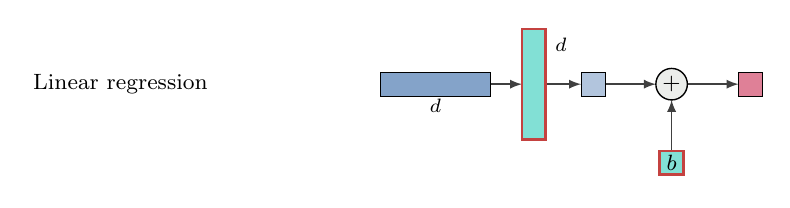
\begin{tikzpicture}
  \begin{scope}[scale=1]
       \Vertex[Math, x=1,y=0, color=xkcdFadedBlue, opacity=.8, shape = rectangle, label = \x, fontsize=\footnotesize, style={minimum width=1.4cm, minimum height=3mm, line width=.1pt}]{B0}
       \Text[position=below,x=1,y=0, distance=1.2mm, fontsize=\scriptsize]{$d$}
       \Vertex[Math, x=2.25,y=0, color=xkcdTurquoise, opacity=.5, shape = rectangle, label = \w, fontsize=\footnotesize, style={minimum width=.3cm, minimum height=1.4cm, line width=1pt,  draw=xkcdReddish}]{B1}
       \Text[position=right,x=2.25,y=.5, distance=2mm, fontsize=\scriptsize]{$d$}
       \Edge[lw=.5pt, Direct](B0)(B1)
       \Vertex[Math, x=3,y=0, color=xkcdFadedBlue, opacity=.5, shape = rectangle, fontsize=\footnotesize, style={minimum width=3mm, minimum height=3mm, line width=.1pt}]{B2}
       \Edge[lw=.5pt, Direct](B1)(B2)
       \Vertex[Math, x=4,y=0, color=xkcdLightGrey, label = +, size = .4, opacity=.5, fontsize=\footnotesize, style={line width=.5pt}]{C}
       \Edge[lw=.5pt, Direct](B2)(C)
       \Vertex[Math, x=4,y=-1, color=xkcdTurquoise, label = b, opacity=.5, shape = rectangle, fontsize=\footnotesize, style={minimum width=3mm, minimum height=3mm, line width=1pt,  draw=xkcdReddish}]{B3}
      \Edge[lw=.5pt, Direct](B3)(C)
      \Vertex[Math, x=5,y=0, color=xkcdLipstickRed, opacity=.5, shape = rectangle, fontsize=\footnotesize, style={minimum width=3mm, minimum height=3mm, line width=.1pt}]{C3}
      \Edge[lw=.5pt, Direct](C)(C3)
      \Text[x=-3,y=0, fontsize=\footnotesize]{Linear regression}
  \end{scope}
  \end{tikzpicture}
  \end{center}
  \medskip
  \begin{itemize}
    \item The last block outputs the affine response directly ($\varphi = \text{identity}$).
    \item No nonlinearity whatsoever: fast and interpretable, but expressiveness is limited to \alert{affine functions} of the input.
  \end{itemize}
\end{frame}

\begin{frame}{Logistic Regression: Adding a Nonlinearity}
  \framesubtitle{Diagram: same affine map, followed by the sigmoid $\sigma$}
  \begin{center}
  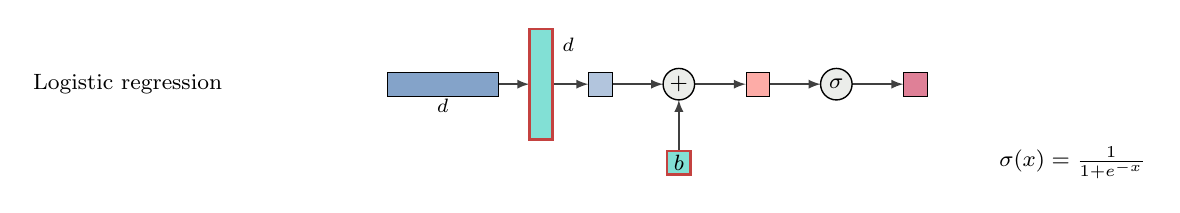
\begin{tikzpicture}
   \begin{scope}[scale=1]
    \Vertex[Math, x=1,y=0, color=xkcdFadedBlue, opacity=.8, shape = rectangle, label = \x, fontsize=\footnotesize, style={minimum width=1.4cm, minimum height=3mm, line width=.1pt}]{B0}
   \Text[position=below,x=1,y=0, distance=1.2mm, fontsize=\scriptsize]{$d$}
   \Vertex[Math, x=2.25,y=0, color=xkcdTurquoise, opacity=.5, shape = rectangle, label =\w, fontsize=\footnotesize, style={minimum width=.3cm, minimum height=1.4cm, line width=1pt,  draw=xkcdReddish}]{B1}
   \Text[position=right,x=2.25,y=.5, distance=2mm, fontsize=\scriptsize]{$d$}
     \Edge[lw=.5pt, Direct](B0)(B1)
  \Vertex[Math, x=3,y=0, color=xkcdFadedBlue, opacity=.5, shape = rectangle, fontsize=\footnotesize, style={minimum width=3mm, minimum height=3mm, line width=.1pt}]{B2}
  \Edge[lw=.5pt, Direct](B1)(B2)
  \Vertex[Math, x=4,y=0, color=xkcdLightGrey, label = +, size = .4, opacity=.5, fontsize=\footnotesize, style={line width=.5pt}]{C}
  \Edge[lw=.5pt, Direct](B2)(C)
  \Vertex[Math, x=4,y=-1, color=xkcdTurquoise, label = b, opacity=.5, shape = rectangle, fontsize=\footnotesize, style={minimum width=3mm, minimum height=3mm, line width=1pt,  draw=xkcdReddish}]{B3}
  \Edge[lw=.5pt, Direct](B3)(C)
  \Vertex[Math, x=5,y=0, color=xkcdCoral, opacity=.5, shape = rectangle, fontsize=\footnotesize, style={minimum width=3mm, minimum height=3mm, line width=.1pt}]{C1}
  \Edge[lw=.5pt, Direct](C)(C1)
  \Vertex[Math, x=6,y=0, color=xkcdLightGrey, label = \sigma, size = .4, opacity=.5, fontsize=\footnotesize, style={line width=.5pt}]{C2}
  \Edge[lw=.5pt, Direct](C1)(C2)
  \Vertex[Math, x=7,y=0, color=xkcdLipstickRed, opacity=.5, shape = rectangle, fontsize=\footnotesize, style={minimum width=3mm, minimum height=3mm, line width=.1pt}]{C3}
  \Edge[lw=.5pt, Direct](C2)(C3)
  \Text[x=9,y=-1, fontsize=\footnotesize]{$\sigma(x)=\frac{1}{1+e^{-x}}$}
  \Text[x=-3,y=0, fontsize=\footnotesize]{Logistic regression}
  \end{scope}
  \end{tikzpicture}
  \end{center}
  \begin{itemize}
    \item One further step: adds the sigmoid, mapping real scores to probabilities in $(0,1)$.
    \item Suitable for \alert{binary classification} — still a single learned affine map.
  \end{itemize}
\end{frame}

\begin{frame}{Softmax Regression: Multiclass Output}
  \framesubtitle{Diagram: weight matrix $\mathbf{W}$ of size $d\times K$, followed by softmax $s$}
  \begin{center}
  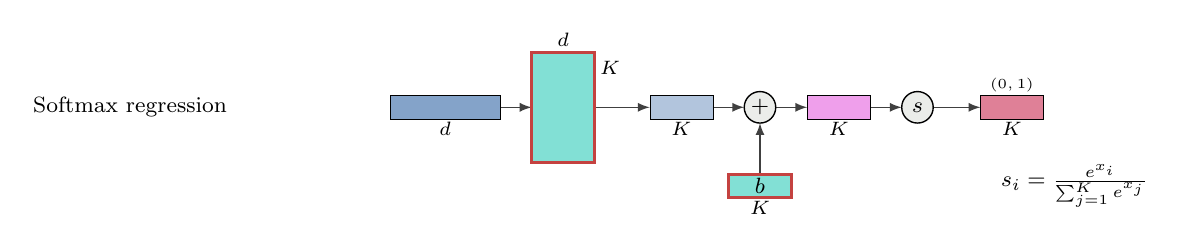
\begin{tikzpicture}
   \begin{scope}[scale=1]
   \Vertex[Math, x=1,y=0, color=xkcdFadedBlue, opacity=.8, shape = rectangle, label = \x, fontsize=\footnotesize, style={minimum width=1.4cm, minimum height=3mm, line width=.1pt}]{B0}
   \Text[position=below,x=1,y=0, distance=1.2mm, fontsize=\scriptsize]{$d$}
   \Vertex[Math, x=2.5,y=0, color=xkcdTurquoise, opacity=.5, shape = rectangle, label = \W, fontsize=\footnotesize, style={minimum width=.8cm, minimum height=1.4cm, line width=1pt,  draw=xkcdReddish}]{B1}
   \Text[position=above,x=2.5,y=0, distance=7mm, fontsize=\scriptsize]{$d$}
   \Text[position=right,x=2.5,y=.5, distance=4mm, fontsize=\scriptsize]{$K$}
   \Edge[lw=.5pt, Direct](B0)(B1)
   \Vertex[Math, x=4,y=0, color=xkcdFadedBlue, opacity=.5, shape = rectangle, fontsize=\footnotesize, style={minimum width=.8cm, minimum height=3mm, line width=.1pt}]{B2}
   \Text[position=below,x=4,y=0, distance=1.2mm, fontsize=\scriptsize]{$K$}
   \Edge[lw=.5pt, Direct](B1)(B2)
   \Vertex[Math, x=5,y=0, color=xkcdLightGrey, label = +, size = .4, opacity=.5, fontsize=\footnotesize, style={line width=.5pt}]{C}
   \Edge[lw=.5pt, Direct](B2)(C)
   \Vertex[Math, x=5,y=-1, color=xkcdTurquoise, label = b, opacity=.5, shape = rectangle, fontsize=\footnotesize, style={minimum width=.8cm, minimum height=3mm, line width=1pt,  draw=xkcdReddish}]{B3}
   \Text[position=below,x=5,y=-1, distance=1.2mm, fontsize=\scriptsize]{$K$}
   \Edge[lw=.5pt, Direct](B3)(C)
   \Vertex[Math, x=6,y=0, color=xkcdPurplePink, opacity=.5, shape = rectangle, fontsize=\footnotesize, style={minimum width=.8cm, minimum height=3mm, line width=.1pt}]{C1}
   \Text[position=below,x=6,y=0, distance=1.2mm, fontsize=\scriptsize]{$K$}
   \Edge[lw=.5pt, Direct](C)(C1)
   \Vertex[Math, x=7,y=0, color=xkcdLightGrey, size=.4, shape = ellipse, label = s, style={line width=.5pt}, opacity=.5, fontsize=\footnotesize]{C2}
   \Edge[lw=.5pt, Direct](C1)(C2)
   \Vertex[Math, x=8.2,y=0, color=xkcdLipstickRed, opacity=.5, shape = rectangle, fontsize=\footnotesize, style={minimum width=.8cm, minimum height=3mm, line width=.1pt}]{C3}
   \Text[position=below,x=8.2,y=0, distance=1.2mm, fontsize=\scriptsize]{$K$}
   \Text[position=above,x=8.2,y=0, distance=1.2mm, fontsize=\tiny]{$(0,1)$}
   \Edge[lw=.5pt, Direct](C2)(C3)
   \Text[x=9,y=-1, fontsize=\footnotesize]{$s_i=\frac{e^{x_i}}{\sum_{j=1}^{K}e^{x_j}}$}
   \Text[x=-3,y=0, fontsize=\footnotesize]{Softmax regression}
   \end{scope}
  \end{tikzpicture}
  \end{center}
  \begin{itemize}
    \item $K$ real-valued scores normalized into a \alert{probability distribution} over classes.
    \item Classes compete for probability mass: higher score for one reduces the others.
  \end{itemize}
\end{frame}

%% ════════════════════════════════════════════════════════════════════════════
\section{Basis Functions and Learnable Features}

\begin{frame}{Predefined Basis Functions}
  \begin{itemize}
    \item A classical enrichment of GLMs: introduce a \alert{fixed feature map} $\Phi\colon\mathbb{R}^d\to\mathbb{R}^m$.
    \item Instead of feeding $\x$ directly, first compute $\Phi(\x)$, then apply a linear model:
    \[
      y(\x) = f\!\left(\w^T\Phi(\x)+b\right).
    \]
    \item Model is still \alert{linear in the parameters}, but can be highly nonlinear in $\x$.
    \item The nonlinearity is embedded in the fixed map $\Phi$, not in the final stage.
  \end{itemize}
  \begin{alertblock}{Limitation}
    $\Phi$ must be chosen \alert{before seeing the data}. A poor choice of features can severely
    handicap the model regardless of how well the final linear layer is trained.
  \end{alertblock}
\end{frame}

\begin{frame}{Basis Function Model: Full Diagram}
  \framesubtitle{$\x \to \Phi \to \boldsymbol\varphi(\x) \to \w \to \text{bias} \to \varphi \to$ output}
  \begin{center}
  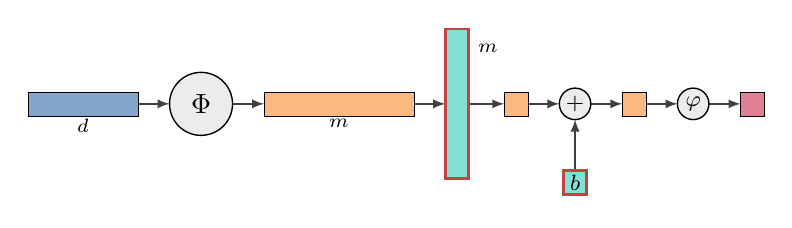
\begin{tikzpicture}
  \Vertex[Math, x=1,y=0, color=xkcdFadedBlue, opacity=.8, shape = rectangle, label = \x, fontsize=\footnotesize, style={minimum width=1.4cm, minimum height=3mm, line width=.1pt}]{B0}
   \Text[position=below,x=1,y=0, distance=1.2mm, fontsize=\scriptsize]{$d$}
  \Vertex[Math, x=2.5,y=0, color=xkcdLightGrey, label = \Phi, size = .8, opacity=.5, fontsize=\normalsize, style={line width=.5pt}]{C}
  \Edge[lw=.5pt, Direct](B0)(C)
  \Vertex[Math, x=4.25,y=0, color=xkcdOrange, opacity=.5, label=\Vphi, shape = rectangle, fontsize=\footnotesize, style={minimum width=1.9cm, minimum height=3mm, line width=.1pt}]{B01}
   \Text[position=below,x=4.25,y=0, distance=1.2mm, fontsize=\scriptsize]{$m$}
   \Edge[lw=.5pt, Direct](C)(B01)
   \Vertex[Math, x=5.75,y=0, color=xkcdTurquoise, opacity=.5, shape = rectangle, label = \w, fontsize=\footnotesize, style={minimum width=.3cm, minimum height=1.9cm, line width=1pt,  draw=xkcdReddish}]{B1}
   \Text[position=right,x=5.75,y=.7, distance=2mm, fontsize=\scriptsize]{$m$}
   \Edge[lw=.5pt, Direct](B01)(B1)
   \Vertex[Math, x=6.5,y=0, color=xkcdOrange, opacity=.5, shape = rectangle, fontsize=\footnotesize, style={minimum width=3mm, minimum height=3mm, line width=.1pt}]{B2}
   \Edge[lw=.5pt, Direct](B1)(B2)
   \Vertex[Math, x=7.25,y=0, color=xkcdLightGrey, label = +, size = .4, opacity=.5, fontsize=\footnotesize, style={line width=.5pt}]{Cadd}
  \Edge[lw=.5pt, Direct](B2)(Cadd)
  \Vertex[Math, x=7.25,y=-1, color=xkcdTurquoise, label = b, opacity=.5, shape = rectangle, fontsize=\footnotesize, style={minimum width=3mm, minimum height=3mm, line width=1pt,  draw=xkcdReddish}]{B3}
  \Vertex[Math, x=8,y=0, color=xkcdOrange, opacity=.5, shape = rectangle, fontsize=\footnotesize, style={minimum width=3mm, minimum height=3mm, line width=.1pt}]{B4}
  \Edge[lw=.5pt, Direct](B3)(Cadd)
  \Edge[lw=.5pt, Direct](Cadd)(B4)
  \Vertex[Math, x=8.75,y=0, color=xkcdLightGrey, label = \varphi, size = .4, opacity=.5, fontsize=\footnotesize, style={line width=.5pt}]{C1}
  \Edge[lw=.5pt, Direct](B4)(C1)
  \Vertex[Math, x=9.5,y=0, color=xkcdLipstickRed, opacity=.5, shape = rectangle, fontsize=\footnotesize, style={minimum width=3mm, minimum height=3mm, line width=.1pt}]{C6}
  \Edge[lw=.5pt, Direct](C1)(C6)
  \end{tikzpicture}
  \end{center}
\end{frame}

\begin{frame}{From Fixed to Learnable Features}
  \begin{itemize}
    \item In the basis-function viewpoint, $\Phi$ is fixed and only $(\w, b)$ are learned.
    \item \textbf{Multilayer networks} arise when we \alert{replace fixed basis functions with learnable ones}.
    \item The role of $\Phi$ is taken by a collection of intermediate GLMs whose parameters are \alert{trained jointly} with the rest of the model.
  \end{itemize}
  \begin{block}{Conceptual shift}
    Rather than engineering features by hand, the network \alert{discovers} from data what
    representations are most useful for the task.
  \end{block}
  \begin{itemize}
    \item This substitution is simple in concept but has \alert{profound consequences} for expressiveness.
  \end{itemize}
\end{frame}

\begin{frame}{One Hidden Layer: The Basic Block}
  \framesubtitle{Diagram: $\x \to \mathbf{W}_1$ (learnable) $\to h_1 \to \w_2 \to \varphi \to$ output}
  \begin{center}
  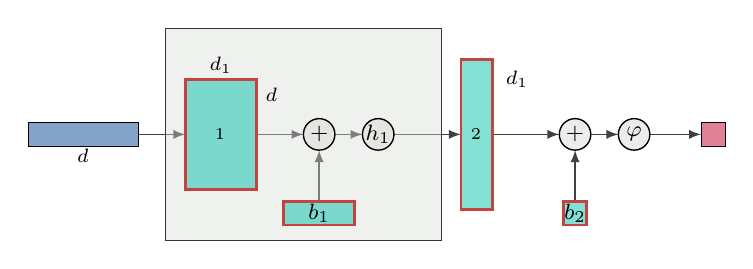
\begin{tikzpicture}
  \begin{scope}
   \Vertex[Math, x=3.8,y=0, color=xkcdLightGrey, opacity=.4, shape = rectangle, style={minimum width=3.5cm, minimum height=2.7cm, line width=.3pt, draw=xkcdDarkGrey}]{A0}
   \Vertex[Math, x=1,y=0, color=xkcdFadedBlue, opacity=.8, shape = rectangle, label = \x, fontsize=\footnotesize, style={minimum width=1.4cm, minimum height=3mm, line width=.1pt}]{B0}
   \Text[position=below,x=1,y=0, distance=1.2mm, fontsize=\scriptsize]{$d$}
   \Vertex[Math, x=2.75,y=0, color=xkcdTurquoise, opacity=.5, shape = rectangle, label = \W_1, fontsize=\footnotesize, style={minimum width=.9cm, minimum height=1.4cm, line width=1pt, draw=xkcdReddish}]{B1}
   \Text[position=above,x=2.75,y=0, distance=7mm, fontsize=\scriptsize]{$d_1$}
   \Text[position=right,x=2.75,y=.5, distance=5mm, fontsize=\scriptsize]{$d$}
   \Edge[lw=.5pt, Direct](B0)(B1)
   \Vertex[Math, x=4,y=0, color=xkcdLightGrey, label = +, size = .4, opacity=.5, fontsize=\footnotesize, style={line width=.5pt}]{C}
   \Edge[lw=.5pt, Direct](B1)(C)
   \Vertex[Math, x=4,y=-1, color=xkcdTurquoise, label = b_1, opacity=.5, shape = rectangle, fontsize=\footnotesize, style={minimum width=9mm, minimum height=3mm, line width=1pt, draw=xkcdReddish}]{B3}
   \Edge[lw=.5pt, Direct](B3)(C)
   \Vertex[Math, x=4.75,y=0, color=xkcdLightGrey, label = h_1, size = .4, opacity=.5, fontsize=\footnotesize, style={line width=.5pt}]{C1}
   \Edge[lw=.5pt, Direct](C)(C1)
   \Vertex[Math, x=6,y=0, color=xkcdTurquoise, opacity=.5, shape = rectangle, label = \w_2, fontsize=\footnotesize, style={minimum width=.4cm, minimum height=1.9cm, line width=1pt, draw=xkcdReddish}]{B4}
   \Text[position=right,x=5.7,y=.7, distance=6mm, fontsize=\scriptsize]{$d_1$}
   \Edge[lw=.5pt, Direct](C1)(B4)
   \Vertex[Math, x=7.25,y=0, color=xkcdLightGrey, label = +, size = .4, opacity=.5, fontsize=\footnotesize, style={line width=.5pt}]{C2}
   \Edge[lw=.5pt, Direct](B4)(C2)
   \Vertex[Math, x=7.25,y=-1, color=xkcdTurquoise, label = b_2, opacity=.5, shape = rectangle, fontsize=\footnotesize, style={minimum width=3mm, minimum height=3mm, line width=1pt, draw=xkcdReddish}]{B5}
   \Edge[lw=.5pt, Direct](B5)(C2)
   \Vertex[Math, x=8,y=0, color=xkcdLightGrey, label = \varphi, size = .4, opacity=.5, fontsize=\footnotesize, style={line width=.5pt}]{C3}
   \Edge[lw=.5pt, Direct](C2)(C3)
   \Vertex[Math, x=9,y=0, color=xkcdLipstickRed, opacity=.5, shape = rectangle, fontsize=\footnotesize, style={minimum width=3mm, minimum height=3mm, line width=.1pt}]{C6}
   \Edge[lw=.5pt, Direct](C3)(C6)
  \end{scope}
  \end{tikzpicture}
  \end{center}
  \begin{itemize}
    \item The grey box represents the \alert{learnable feature extraction block} (first layer).
    \item $\mathbf{W}_1$ is now trained jointly with $\w_2$.
  \end{itemize}
\end{frame}

%% ════════════════════════════════════════════════════════════════════════════
\section{The Hidden Layer: Activations and Nonlinearities}

\begin{frame}{Pre-activations and the Hidden Layer}
  \begin{itemize}
    \item From input $\x = (x_1,\ldots,x_d)$, the first layer produces $d_1$ \alert{activations}:
    \[
      a_j = \sum_{i=1}^{d} w_{ji} x_i + b_j = \overline{\w}_j^T \overline{\x}.
    \]
    \item $a_j$ is called a \alert{pre-activation}: the value to be transformed before being passed on.
    \item Each unit has its own weight vector and bias; the layer computes $d_1$ affine functions simultaneously.
  \end{itemize}
  \begin{block}{Activation function}
    Each pre-activation is passed through a nonlinear function $h_1$:
    \[
      z_j = h_1(a_j) = h_1\!\left(\w_j^T\x + b_j\right).
    \]
    The vector $\z = (z_1,\ldots,z_{d_1})$ is the representation produced by the first layer.
  \end{block}
\end{frame}

\begin{frame}{Why Nonlinearity Is Necessary}
  \begin{itemize}
    \item Without nonlinearities between layers, \alert{composing any number of affine maps} simply produces another affine map.
    \item Increasing depth would add \alert{no expressive power} beyond what a single linear layer achieves.
    \item The nonlinearity is therefore what makes depth \alert{meaningful}.
    \item In practice $h_1$ is often chosen as an approximate thresholding mechanism:
      \begin{itemize}
        \item Saturates for large positive and large negative inputs.
        \item Produces outputs near two different extreme values.
        \item Varies smoothly in between.
      \end{itemize}
  \end{itemize}
\end{frame}

\begin{frame}{Classical Activation Functions}
  \begin{columns}[t]
    \column{0.48\textwidth}
      \begin{block}{Sigmoid}
        \[
          \sigma(x) = \frac{1}{1+e^{-x}}
        \]
        \begin{itemize}
          \item Output in $(0,1)$.
          \item Smooth ``S-shaped'' curve.
        \end{itemize}
      \end{block}
    \column{0.48\textwidth}
      \begin{block}{Hyperbolic Tangent}
        \[
          \tanh(x) = \frac{e^x - e^{-x}}{e^x + e^{-x}}
        \]
        \begin{itemize}
          \item Output in $(-1,1)$: \alert{centered at zero}.
          \item $\tanh(x) = \sigma(2x) - \sigma(-2x)$.
        \end{itemize}
      \end{block}
  \end{columns}
  \medskip
  \begin{itemize}
    \item The identity $\tanh(x)=\sigma(2x)-\sigma(-2x)$ reveals qualitatively similar saturating behavior.
    \item Centering around zero makes $\tanh$ more convenient in hidden layers: positive and negative activations are treated more symmetrically.
  \end{itemize}
\end{frame}

\begin{frame}{Figure: First Layer Computation}
  \framesubtitle{From augmented input to activations $z_1^{(1)},\ldots,z_{d_1}^{(1)}$}
  \begin{center}
  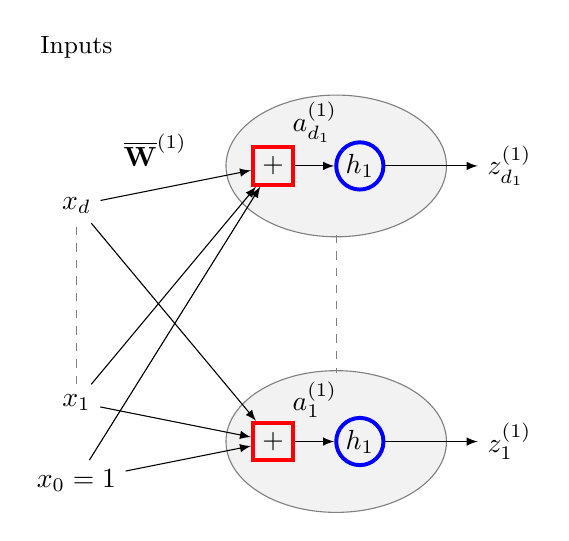
\begin{tikzpicture}[>=latex]
    \node (Label01) at (1,-1)  {$x_{0}=1$};
    \node (Label11) at (1, 0)  {$x_{1}$};
    \node (Labeld1) at (1, 2.5){$x_{d}$};
    \node (Label1)  at (1, 4.5){\small Inputs};
    \fill[lightgray!20] (4.3,-.5) ellipse (1.4 and .9);
    \fill[lightgray!20] (4.3, 3)  ellipse (1.4 and .9);
    \draw[gray] (4.3,-.5) ellipse (1.4 and .9);
    \draw[gray] (4.3, 3)  ellipse (1.4 and .9);
    \node[draw=red, line width=.5mm, inner sep=1.2mm] (Add12) at (3.5,-.5) {$+$};
    \node[draw=red, line width=.5mm, inner sep=1.2mm] (Addm2) at (3.5, 3)  {$+$};
    \node[draw=blue, line width=.5mm, circle, minimum size=6mm, inner sep=0pt] (Act12) at (4.6,-.5) {$h_{1}$};
    \node[draw=blue, line width=.5mm, circle, minimum size=6mm, inner sep=0pt] (Actm2) at (4.6, 3)  {$h_{1}$};
    \node (Label12) at (6.5,-.5) {$z_{1}^{(1)}$};
    \node (Label0m) at (6.5, 3)  {$z_{d_1}^{(1)}$};
    \node (n1) at (4.3, 2.25) {};
    \node (n2) at (4.3, 0.25) {};
    \node (beta1) at (2, 3.2) {$\mathbf{\overline{W}}^{(1)}$};
    \draw[->] (Label01) -- (Add12);
    \draw[->] (Label01) -- (Addm2);
    \draw[->] (Label11) -- (Add12);
    \draw[->] (Label11) -- (Addm2);
    \draw[->] (Labeld1) -- (Add12);
    \draw[->] (Labeld1) -- (Addm2);
    \draw[->] (Addm2) -- node[above=5pt] {$a_{d_1}^{(1)}$} (Actm2);
    \draw[->] (Add12) -- node[above=5pt] {$a_{1}^{(1)}$}   (Act12);
    \draw[->] (Act12) -- (Label12);
    \draw[->] (Actm2) -- (Label0m);
    \draw[gray, dashed] (Label11) -- (Labeld1);
    \draw[gray, dashed] (n1)      -- (n2);
  \end{tikzpicture}
  \end{center}
\end{frame}

%% ════════════════════════════════════════════════════════════════════════════
\section{Multilayer Architecture}

\begin{frame}{Stacking Layers: The Idea of Depth}
  \begin{itemize}
    \item Once the first layer produces $\z^{(1)}$, the \alert{same construction can be iterated}.
    \item Feed $\z^{(1)}$ into a second layer of units; compute new pre-activations and outputs.
    \item By stacking several layers, we obtain a \alert{multilayer network}.
    \item The depth is precisely the number of times the affine-then-nonlinear pattern is repeated.
  \end{itemize}
  \begin{block}{General layer $r$ computation}
    \[
      a_k^{(r)} = \overline{\w}_k^{(r)T}\overline{\z}^{(r-1)}, \qquad
      z_k^{(r)} = h_r\!\left(\overline{\w}_k^{(r)T}\overline{\z}^{(r-1)}\right).
    \]
  \end{block}
  \begin{itemize}
    \item $\overline{\z}^{(r-1)}$ denotes the augmented vector including the bias unit.
    \item Each hidden unit is a small GLM acting on the \alert{features of the previous layer}.
  \end{itemize}
\end{frame}

\begin{frame}{Figure: Two Hidden Layers}
  \framesubtitle{Adding a second hidden layer to the basic architecture}
  \begin{center}
  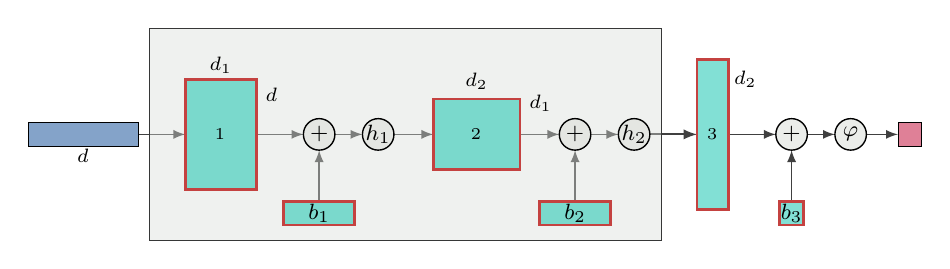
\begin{tikzpicture}
       \Vertex[Math, x=5.1,y=0, color=xkcdLightGrey, opacity=.4, shape = rectangle, style={minimum width=6.5cm, minimum height=2.7cm, line width=.3pt, draw=xkcdDarkGrey}]{A0}
  \Vertex[Math, x=1,y=0, color=xkcdFadedBlue, opacity=.8, shape = rectangle, label = \x, fontsize=\footnotesize, style={minimum width=1.4cm, minimum height=3mm, line width=.1pt}]{B0}
   \Text[position=below,x=1,y=0, distance=1.2mm, fontsize=\scriptsize]{$d$}
   \Vertex[Math, x=2.75,y=0, color=xkcdTurquoise, opacity=.5, shape = rectangle, label = \W_1, fontsize=\footnotesize, style={minimum width=.9cm, minimum height=1.4cm, line width=1pt, draw=xkcdReddish}]{B1}
   \Text[position=above,x=2.75,y=0, distance=7mm, fontsize=\scriptsize]{$d_1$}
   \Text[position=right,x=2.75,y=.5, distance=5mm, fontsize=\scriptsize]{$d$}
   \Edge[lw=.5pt, Direct](B0)(B1)
   \Vertex[Math, x=4,y=0, color=xkcdLightGrey, label = +, size = .4, opacity=.5, fontsize=\footnotesize, style={line width=.5pt}]{C}
   \Edge[lw=.5pt, Direct](B1)(C)
   \Vertex[Math, x=4,y=-1, color=xkcdTurquoise, label = b_1, opacity=.5, shape = rectangle, fontsize=\footnotesize, style={minimum width=9mm, minimum height=3mm, line width=1pt, draw=xkcdReddish}]{B3}
   \Edge[lw=.5pt, Direct](B3)(C)
   \Vertex[Math, x=4.75,y=0, color=xkcdLightGrey, label = h_1, size = .4, opacity=.5, fontsize=\footnotesize, style={line width=.5pt}]{C1}
   \Edge[lw=.5pt, Direct](C)(C1)
   \Vertex[Math, x=6,y=0, color=xkcdTurquoise, opacity=.5, shape = rectangle, label = \W_2, fontsize=\footnotesize, style={minimum width=1.1cm, minimum height=.9cm, line width=1pt, draw=xkcdReddish}]{B4}
   \Text[position=above,x=6,y=0, distance=5mm, fontsize=\scriptsize]{$d_2$}
   \Text[position=right,x=6,y=.4, distance=6mm, fontsize=\scriptsize]{$d_1$}
   \Edge[lw=.5pt, Direct](C1)(B4)
   \Vertex[Math, x=7.25,y=0, color=xkcdLightGrey, label = +, size = .4, opacity=.5, fontsize=\footnotesize, style={line width=.5pt}]{C2}
   \Edge[lw=.5pt, Direct](B4)(C2)
   \Vertex[Math, x=7.25,y=-1, color=xkcdTurquoise, label = b_2, opacity=.5, shape = rectangle, fontsize=\footnotesize, style={minimum width=9mm, minimum height=3mm, line width=1pt, draw=xkcdReddish}]{B5}
   \Edge[lw=.5pt, Direct](B5)(C2)
   \Vertex[Math, x=8,y=0, color=xkcdLightGrey, label = h_2, size = .4, opacity=.5, fontsize=\footnotesize, style={line width=.5pt}]{C3}
   \Edge[lw=.5pt, Direct](C2)(C3)
   \Vertex[Math, x=9,y=0, color=xkcdTurquoise, opacity=.5, shape = rectangle, label = \w_3, fontsize=\footnotesize, style={minimum width=.4cm, minimum height=1.9cm, line width=1pt, draw=xkcdReddish}]{B41}
   \Text[position=right,x=9,y=.7, distance=2mm, fontsize=\scriptsize]{$d_2$}
   \Edge[lw=.7pt, Direct](C3)(B41)
   \Vertex[Math, x=10,y=0, color=xkcdLightGrey, label = +, size = .4, opacity=.5, fontsize=\footnotesize, style={line width=.5pt}]{C21}
   \Edge[lw=.5pt, Direct](B41)(C21)
   \Vertex[Math, x=10,y=-1, color=xkcdTurquoise, label = b_3, opacity=.5, shape = rectangle, fontsize=\footnotesize, style={minimum width=3mm, minimum height=3mm, line width=1pt, draw=xkcdReddish}]{B51}
   \Edge[lw=.5pt, Direct](B51)(C21)
   \Vertex[Math, x=10.75,y=0, color=xkcdLightGrey, label = \varphi, size = .4, opacity=.5, fontsize=\footnotesize, style={line width=.5pt}]{C31}
   \Edge[lw=.5pt, Direct](C21)(C31)
   \Vertex[Math, x=11.5,y=0, color=xkcdLipstickRed, opacity=.5, shape = rectangle, fontsize=\footnotesize, style={minimum width=3mm, minimum height=3mm, line width=.1pt}]{C6}
   \Edge[lw=.5pt, Direct](C31)(C6)
  \end{tikzpicture}
  \end{center}
\end{frame}

\begin{frame}{Figure: A Generic Hidden Layer $r$}
  \framesubtitle{Inputs $z^{(r-1)}$ to outputs $z^{(r)}$ via pre-activations $a^{(r)}$}
  \begin{center}
  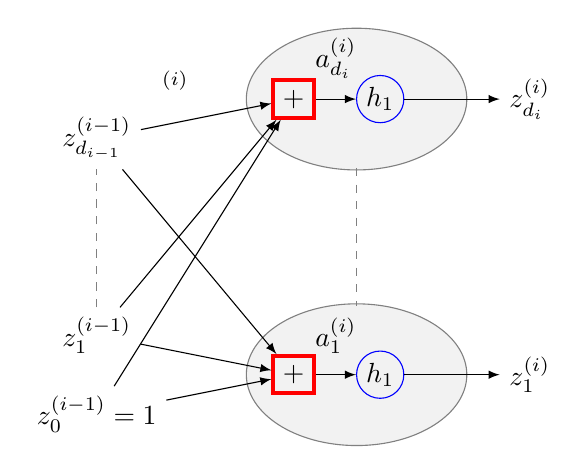
\begin{tikzpicture}[>=latex]
    \node (Label01) at (1,-1)  {$z_{0}^{(i-1)}=1$};
    \node (Label11) at (1, 0)  {$z_{1}^{(i-1)}$};
    \node (Labeld1) at (1, 2.5){$z_{d_{i-1}}^{(i-1)}$};
    \fill[lightgray!20] (4.3,-.5) ellipse (1.4 and .9);
    \fill[lightgray!20] (4.3, 3)  ellipse (1.4 and .9);
    \draw[gray] (4.3,-.5) ellipse (1.4 and .9);
    \draw[gray] (4.3, 3)  ellipse (1.4 and .9);
    \node[draw=red, line width=.5mm, inner sep=1.2mm] (Add12) at (3.5,-.5) {$+$};
    \node[draw=red, line width=.5mm, inner sep=1.2mm] (Addm2) at (3.5, 3)  {$+$};
    \node[draw=blue, circle, minimum size=6mm, inner sep=0pt] (Act12) at (4.6,-.5) {$h_{1}$};
    \node[draw=blue, circle, minimum size=6mm, inner sep=0pt] (Actm2) at (4.6, 3)  {$h_{1}$};
    \node (Label12) at (6.5,-.5) {$z_{1}^{(i)}$};
    \node (Label0m) at (6.5, 3)  {$z_{d_i}^{(i)}$};
    \node (n1) at (4.3, 2.25) {};
    \node (n2) at (4.3, 0.25) {};
    \node (beta1) at (2, 3.2) {$\overline{\W}^{(i)}$};
    \draw[->] (Label01) -- (Add12);
    \draw[->] (Label01) -- (Addm2);
    \draw[->] (Label11) -- (Add12);
    \draw[->] (Label11) -- (Addm2);
    \draw[->] (Labeld1) -- (Add12);
    \draw[->] (Labeld1) -- (Addm2);
    \draw[->] (Addm2) -- node[above=4pt] {$a_{d_i}^{(i)}$} (Actm2);
    \draw[->] (Add12) -- node[above=4pt] {$a_{1}^{(i)}$}   (Act12);
    \draw[->] (Act12) -- (Label12);
    \draw[->] (Actm2) -- (Label0m);
    \draw[gray, dashed] (Label11) -- (Labeld1);
    \draw[gray, dashed] (n1)      -- (n2);
  \end{tikzpicture}
  \end{center}
\end{frame}

\begin{frame}{The Output Layer}
  \begin{itemize}
    \item After $D-1$ hidden layers, the final layer $D$ produces the network output $\y = \z^{(D)}$.
    \item Same pattern: affine combination of the previous layer's outputs, then a nonlinearity $\varphi$.
    \[
      a_k^{(D)} = \overline{\w}_k^{(D)T}\overline{\z}^{(D-1)}, \qquad
      y_k = z_k^{(D)} = \varphi\!\left(\overline{\w}_k^{(D)T}\overline{\z}^{(D-1)}\right).
    \]
    \item $\varphi$ is chosen based on the \alert{task requirements}, not representational convenience.
  \end{itemize}
  \begin{block}{Choice of output function $\varphi$}
    \begin{tabular}{ll}
      \textbf{Regression} & Identity ($\varphi(x)=x$): output in $\mathbb{R}$ \\
      \textbf{Binary classification} & Sigmoid: output in $(0,1)$, interpreted as probability \\
      \textbf{$K$-class classification} & Softmax: outputs form a valid probability vector
    \end{tabular}
  \end{block}
\end{frame}

\begin{frame}{Output Layer: Regression}
  \framesubtitle{Identity output — linear regression on the final representation}
  \begin{center}
  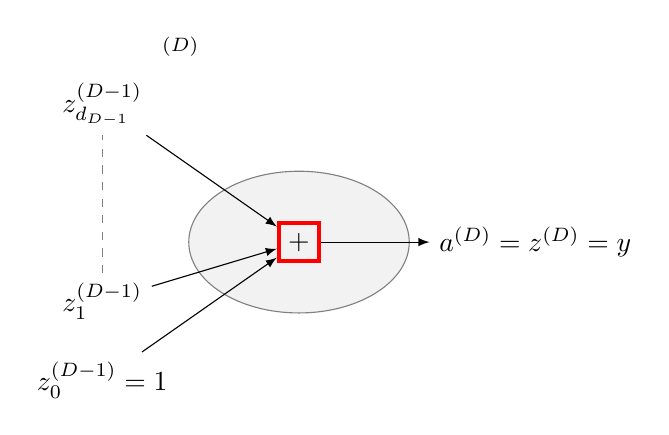
\begin{tikzpicture}[>=latex]
    \node (Label01) at (1,-1)  {$z_{0}^{(D-1)}=1$};
    \node (Label11) at (1, 0)  {$z_{1}^{(D-1)}$};
    \node (Labeld1) at (1, 2.5){$z_{d_{D-1}}^{(D-1)}$};
    \fill[lightgray!20] (3.5,.75) ellipse (1.4 and .9);
    \draw[gray] (3.5,.75) ellipse (1.4 and .9);
    \node[draw=red, line width=.5mm, inner sep=1.2mm] (Add12) at (3.5,.75) {$+$};
    \node (Label12) at (6.5,.75) {$a^{(D)}=z^{(D)}=y$};
    \node (beta1) at (2, 3.2) {$\overline{\w}^{(D)}$};
    \draw[->] (Label01) -- (Add12);
    \draw[->] (Label11) -- (Add12);
    \draw[->] (Labeld1) -- (Add12);
    \draw[->] (Add12) -- (Label12);
    \draw[gray, dashed] (Label11) -- (Labeld1);
  \end{tikzpicture}
  \end{center}
  \begin{itemize}
    \item No nonlinearity node: $y = a^{(D)} = \overline{\w}^{(D)T}\overline{\z}^{(D-1)}$.
    \item Equivalent to linear regression \alert{applied to the learned representation} $\z^{(D-1)}$.
  \end{itemize}
\end{frame}

\begin{frame}{Output Layer: Binary Classification}
  \framesubtitle{Sigmoid output — probability in $(0,1)$}
  \begin{center}
  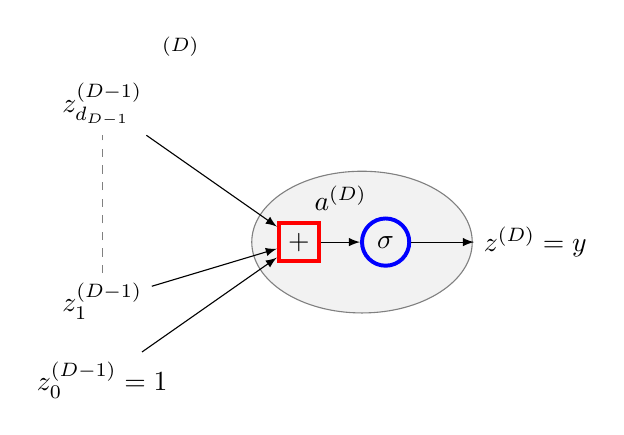
\begin{tikzpicture}[>=latex]
    \node (Label01) at (1,-1)  {$z_{0}^{(D-1)}=1$};
    \node (Label11) at (1, 0)  {$z_{1}^{(D-1)}$};
    \node (Labeld1) at (1, 2.5){$z_{d_{D-1}}^{(D-1)}$};
    \fill[lightgray!20] (4.3,.75) ellipse (1.4 and .9);
    \draw[gray] (4.3,.75) ellipse (1.4 and .9);
    \node[draw=red, line width=.5mm, inner sep=1.2mm] (Add12) at (3.5,.75) {$+$};
    \node[draw=blue, line width=.5mm, circle, minimum size=6mm, inner sep=0pt] (Act12) at (4.6,.75) {$\sigma$};
    \node (Label12) at (6.5,.75) {$z^{(D)}=y$};
    \node (beta1) at (2, 3.2) {$\overline{\w}^{(D)}$};
    \draw[->] (Label01) -- (Add12);
    \draw[->] (Label11) -- (Add12);
    \draw[->] (Labeld1) -- (Add12);
    \draw[->] (Add12) -- node[above=8pt] {$a^{(D)}$} (Act12);
    \draw[->] (Act12) -- (Label12);
    \draw[gray, dashed] (Label11) -- (Labeld1);
  \end{tikzpicture}
  \end{center}
  \begin{itemize}
    \item The affine score $a^{(D)}$ is squashed to $(0,1)$ by $\sigma$.
    \item Probabilistic interpretation: estimated probability that the input belongs to the positive class.
    \item Tied naturally to the \alert{cross-entropy loss} (Bernoulli model).
  \end{itemize}
\end{frame}

\begin{frame}{Output Layer: $K$-Class Classification}
  \framesubtitle{Softmax output — probability vector over $K$ classes}
  \begin{center}
  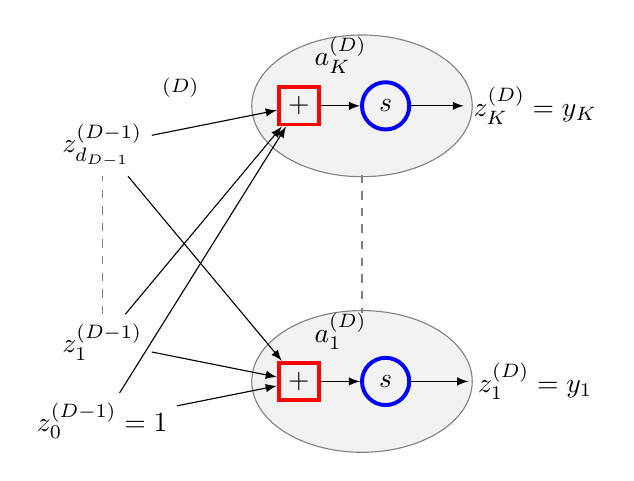
\begin{tikzpicture}[>=latex]
    \node (Label01) at (1,-1)  {$z_{0}^{(D-1)}=1$};
    \node (Label11) at (1, 0)  {$z_{1}^{(D-1)}$};
    \node (Labeld1) at (1, 2.5){$z_{d_{D-1}}^{(D-1)}$};
    \fill[lightgray!20] (4.3,-.5) ellipse (1.4 and .9);
    \fill[lightgray!20] (4.3, 3)  ellipse (1.4 and .9);
    \draw[gray] (4.3,-.5) ellipse (1.4 and .9);
    \draw[gray] (4.3, 3)  ellipse (1.4 and .9);
    \node[draw=red, line width=.5mm, inner sep=1.2mm] (Add12) at (3.5,-.5) {$+$};
    \node[draw=red, line width=.5mm, inner sep=1.2mm] (Addm2) at (3.5, 3)  {$+$};
    \node[draw=blue, line width=.5mm, circle, minimum size=6mm, inner sep=0pt] (Act12) at (4.6,-.5) {$s$};
    \node[draw=blue, line width=.5mm, circle, minimum size=6mm, inner sep=0pt] (Actm2) at (4.6, 3)  {$s$};
    \node (Label12) at (6.5,-.5) {$z_{1}^{(D)}=y_1$};
    \node (Label0m) at (6.5, 3)  {$z_{K}^{(D)}=y_K$};
    \node (n1) at (4.3, 2.25) {};
    \node (n2) at (4.3, 0.25) {};
    \node (beta1) at (2, 3.2) {$\overline{\W}^{(D)}$};
    \draw[->] (Label01) -- (Add12);
    \draw[->] (Label01) -- (Addm2);
    \draw[->] (Label11) -- (Add12);
    \draw[->] (Label11) -- (Addm2);
    \draw[->] (Labeld1) -- (Add12);
    \draw[->] (Labeld1) -- (Addm2);
    \draw[->] (Addm2) -- node[above=8pt] {$a_{K}^{(D)}$} (Actm2);
    \draw[->] (Add12) -- node[above=8pt] {$a_{1}^{(D)}$}  (Act12);
    \draw[->] (Act12) -- (Label12);
    \draw[->] (Actm2) -- (Label0m);
    \draw[gray, dashed] (Label11) -- (Labeld1);
    \draw[gray, dashed] (n1)      -- (n2);
  \end{tikzpicture}
  \end{center}
\end{frame}

\begin{frame}{Softmax: Competition Between Classes}
  \begin{itemize}
    \item $K$ output units, each computing a score (logit) $a_k^{(D)}$ for class $k$.
    \item Softmax normalizes these into a probability vector:
    \[
      y_k = s_k\!\left(a_1^{(D)}, \ldots, a_K^{(D)}\right) = \frac{e^{a_k^{(D)}}}{\displaystyle\sum_{j=1}^{K} e^{a_j^{(D)}}}.
    \]
    \item All outputs are nonnegative and sum to one.
    \item Increasing one class score \alert{reduces the probability} allocated to the others.
    \item Natural companion: \alert{multiclass cross-entropy loss} (categorical distribution MLE).
  \end{itemize}
\end{frame}

%% ════════════════════════════════════════════════════════════════════════════
\section{Three-Layer Networks}

\begin{frame}{The Three-Layer Architecture}
  \begin{itemize}
    \item Input layer + \alert{one hidden layer} + output layer.
    \item Despite the apparent modesty of one hidden layer, already \alert{highly expressive}:
      \begin{itemize}
        \item Hidden layer learns data-dependent nonlinear features tailored to the task.
      \end{itemize}
    \item Natural first step beyond classical GLMs.
  \end{itemize}
  \begin{block}{Three-layer network for $K$-class classification}
    \[
      y_k = s\!\left(\sum_{j=1}^{d_1} w_{kj}^{(2)}\, h\!\left(\sum_{i=1}^{d} w_{ji}^{(1)} x_i + b_j^{(1)}\right) + b_k^{(2)}\right), \quad k=1,\ldots,K.
    \]
  \end{block}
  \begin{itemize}
    \item $d_1$: number of hidden units (structural hyperparameter).
    \item $s$: softmax function.
  \end{itemize}
\end{frame}

\begin{frame}{Three-Layer Network: Reading the Formula Inside Out}
  \begin{enumerate}
    \item \textbf{Inner sum:} $\displaystyle\sum_{i=1}^{d} w_{ji}^{(1)} x_i + b_j^{(1)}$ — pre-activation of hidden unit $j$.
    \item \textbf{Nonlinearity:} $h(\cdot)$ applied to each pre-activation — $j$-th hidden unit output.
    \item \textbf{Outer sum:} $\displaystyle\sum_{j=1}^{d_1} w_{kj}^{(2)}\, h(\cdots) + b_k^{(2)}$ — class-$k$ score from hidden units.
    \item \textbf{Softmax:} $s(\cdot)$ converts $K$ scores into a probability vector.
  \end{enumerate}
  \medskip
  \begin{block}{Unified interpretation}
    The three-layer network is a GLM in which the basis functions
    $h\!\left(\sum_i w_{ji}^{(1)} x_i + b_j^{(1)}\right)$ are \alert{learned from data} through $\overline{\W}^{(1)}$,
    rather than fixed in advance. Features and classifier are \alert{optimized jointly}.
  \end{block}
\end{frame}

\begin{frame}{Figure: Three-Layer Network (Input, Hidden, Output)}
  \framesubtitle{Complete diagram with weight matrices $\overline{\W}^{(1)}$ and $\overline{\W}^{(2)}$}
  \begin{center}
  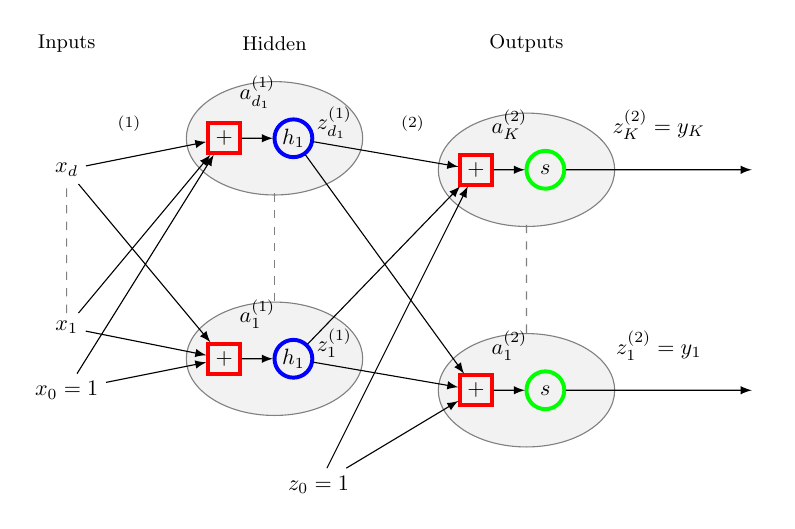
\begin{tikzpicture}[>=latex, scale=0.8, every node/.style={scale=0.8}]
    \node (Label1)  at (-2, 4.5) {\small Inputs};
    \node (Label2)  at (1.3, 4.5) {\small Hidden};
    \node (Label3)  at (5.3, 4.5) {\small Outputs};
    \node (Label01) at (-2,-1)  {$x_{0}=1$};
    \node (Label11) at (-2, 0)  {$x_{1}$};
    \node (Labeld1) at (-2, 2.5){$x_{d}$};
    \node (Label02) at (2,-2.5) {$z_{0}=1$};
    \fill[lightgray!20] (1.3,-.5)  ellipse (1.4 and .9);
    \fill[lightgray!20] (1.3, 3)   ellipse (1.4 and .9);
    \fill[lightgray!20] (5.3, 2.5) ellipse (1.4 and .9);
    \fill[lightgray!20] (5.3,-1)   ellipse (1.4 and .9);
    \draw[gray] (1.3,-.5)  ellipse (1.4 and .9);
    \draw[gray] (1.3, 3)   ellipse (1.4 and .9);
    \draw[gray] (5.3, 2.5) ellipse (1.4 and .9);
    \draw[gray] (5.3,-1)   ellipse (1.4 and .9);
    \node[draw=red, line width=.5mm, inner sep=1.2mm] (Add12) at (.5,-.5) {$+$};
    \node[draw=red, line width=.5mm, inner sep=1.2mm] (Addm2) at (.5, 3)  {$+$};
    \node[draw=red, line width=.5mm, inner sep=1.2mm] (Addk3) at (4.5, 2.5) {$+$};
    \node[draw=red, line width=.5mm, inner sep=1.2mm] (Add13) at (4.5,-1)   {$+$};
    \node[draw=blue, line width=.5mm, circle, minimum size=6mm, inner sep=0pt] (Act12) at (1.6,-.5) {$h_{1}$};
    \node[draw=blue, line width=.5mm, circle, minimum size=6mm, inner sep=0pt] (Actm2) at (1.6, 3)  {$h_{1}$};
    \node[draw=green, line width=.5mm, circle, minimum size=6mm, inner sep=0pt] (Actk3) at (5.6, 2.5) {$s$};
    \node[draw=green, line width=.5mm, circle, minimum size=6mm, inner sep=0pt] (Act13) at (5.6,-1)   {$s$};
    \node (Label12) at (2.25,-.25)  {$z_{1}^{(1)}$};
    \node (Label0m) at (2.25, 3.25) {$z_{d_1}^{(1)}$};
    \node (Outputk) at (9, 2.5) {};
    \node (Output1) at (9,-1)   {};
    \node (n1) at (1.3, 2.25) {};
    \node (n2) at (1.3, 0.25) {};
    \node (n3) at (5.3, 1.75) {};
    \node (n4) at (5.3,-.25)  {};
    \node (beta1) at (-1,  3.2) {$\overline{\W}^{(1)}$};
    \node (beta2) at (3.5, 3.2) {$\overline{\W}^{(2)}$};
    \draw[->] (Label01) -- (Add12); \draw[->] (Label01) -- (Addm2);
    \draw[->] (Label11) -- (Add12); \draw[->] (Label11) -- (Addm2);
    \draw[->] (Labeld1) -- (Add12); \draw[->] (Labeld1) -- (Addm2);
    \draw[->] (Addm2) -- node[above=8pt] {$a_{d_1}^{(1)}$} (Actm2);
    \draw[->] (Add12) -- node[above=8pt] {$a_{1}^{(1)}$}   (Act12);
    \draw[->] (Addk3) -- node[above=8pt] {$a_{K}^{(2)}$} (Actk3);
    \draw[->] (Add13) -- node[above=8pt] {$a_{1}^{(2)}$}  (Act13);
    \draw[->] (Act13) -- node[above=8pt] {$z_{1}^{(2)}=y_{1}$} (Output1);
    \draw[->] (Actk3) -- node[above=8pt] {$z_{K}^{(2)}=y_{K}$} (Outputk);
    \draw[->] (Act12) -- (Add13); \draw[->] (Act12) -- (Addk3);
    \draw[->] (Actm2) -- (Add13); \draw[->] (Actm2) -- (Addk3);
    \draw[->] (Label02) -- (Add13); \draw[->] (Label02) -- (Addk3);
    \draw[gray, dashed] (Label11) -- (Labeld1);
    \draw[gray, dashed] (n1) -- (n2);
    \draw[gray, dashed] (n3) -- (n4);
  \end{tikzpicture}
  \end{center}
\end{frame}

%% ════════════════════════════════════════════════════════════════════════════
\section{Universal Approximation}

\begin{frame}{Neural Networks as Universal Approximators}
  \begin{itemize}
    \item Despite the simplicity of individual units, multilayer networks are \alert{universal approximators}.
    \item Expressive power does not reside in any single unit; it \alert{emerges from their combination}.
  \end{itemize}
  \begin{block}{Universal Approximation Theorem (informal)}
    A feedforward neural network with a \alert{single hidden layer} and a non-polynomial activation
    function can approximate \emph{any} continuous function on a compact domain to arbitrary precision.
  \end{block}
  \begin{itemize}
    \item Depth beyond one hidden layer is not \alert{in principle} necessary for expressiveness.
    \item Width alone suffices — but the required number of units may grow rapidly.
  \end{itemize}
\end{frame}

\begin{frame}{Universal Approximation Theorem: Formal Statement}
  Let $f\colon\mathbb{R}^d\to\mathbb{R}$ be continuous on a compact set $K\subset\mathbb{R}^d$, and let $\varepsilon>0$.\\[0.5em]
  Then there exist $d_1>0$ and parameters $\{w_{ji}^{(1)}, b_j^{(1)}, w_j^{(2)}, b^{(2)}\}$ such that
  \[
    \hat f(\x) = \sum_{j=1}^{d_1} w_j^{(2)}\, h\!\left(\sum_{i=1}^{d} w_{ji}^{(1)} x_i + b_j^{(1)}\right) + b^{(2)}
  \]
  satisfies
  \[
    \sup_{\x\in K} |f(\x) - \hat f(\x)| < \varepsilon,
  \]
  where $h$ is a sigmoidal activation function (e.g., logistic sigmoid or $\tanh$).
\end{frame}

\begin{frame}{Intuition: Hidden Units as Feature Detectors}
  \begin{itemize}
    \item Each hidden unit computes $h(\w^T\x + b)$.
    \item For sigmoidal activations: behaves like a \alert{smooth step function}, transitioning across the hyperplane $\{\x : \w^T\x + b = 0\}$.
    \item By choosing $\w$ and $b$, each unit can be made sensitive to a \alert{particular linear feature} in a specific region of the input domain.
    \item Combining many units through the outer sum constructs a rich set of basis functions.
  \end{itemize}
  \begin{alertblock}{Key advantage over fixed basis functions}
    The directions $\w_j^{(1)}$ and thresholds $b_j^{(1)}$ are \alert{learned from data}: the span of
    the basis functions becomes increasingly dense as $d_1$ grows.
  \end{alertblock}
\end{frame}

\begin{frame}{Limitations and Extensions of the Theorem}
  \begin{columns}[t]
    \column{0.48\textwidth}
      \begin{alertblock}{What the theorem says}
        \begin{itemize}
          \item \textbf{Existence} result only.
          \item Good parameters \alert{exist} for any $f$ and $\varepsilon$.
          \item Says nothing about \alert{how to find} them.
          \item No bound on the required $d_1$.
        \end{itemize}
      \end{alertblock}
    \column{0.48\textwidth}
      \begin{block}{Extensions}
        \begin{itemize}
          \item Analogous guarantees for ReLU and other activations.
          \item Deep networks often achieve comparable approximation with \alert{far fewer total units}.
          \item Depth exploits compositional and hierarchical structure.
        \end{itemize}
      \end{block}
  \end{columns}
  \medskip
  \begin{itemize}
    \item In practice: optimization challenges, regularization, and generalization go beyond the theorem's scope.
  \end{itemize}
\end{frame}

%% ════════════════════════════════════════════════════════════════════════════
\section{Error Functions and Optimization}

\begin{frame}{The Optimization Problem}
  \begin{itemize}
    \item Learning reduces to finding $\overline{\W}$ minimizing an \alert{error function} $E(\overline{\W})$.
    \item $E(\overline{\W})$ is typically \alert{highly nonconvex}: complicated geometry with:
      \begin{itemize}
        \item Many local minima.
        \item Flat regions and saddle points.
        \item Valleys with different depths.
      \end{itemize}
    \item No closed-form solution (unlike linear regression with normal equations).
    \item Must resort to \alert{iterative optimization methods}.
  \end{itemize}
  \begin{block}{Iterative update scheme}
    \[
      \overline{\W}^{(k+1)} = \overline{\W}^{(k)} + \Delta\overline{\W}^{(k)},
    \]
    where $\Delta\overline{\W}^{(k)}$ is chosen so that $E(\overline{\W}^{(k+1)}) < E(\overline{\W}^{(k)})$.
  \end{block}
\end{frame}

\begin{frame}{Non-Uniqueness of Minima}
  \begin{itemize}
    \item For neural networks, local minima are often \alert{not unique} in a meaningful sense.
    \item Two classical symmetries generate equivalent solutions:
  \end{itemize}
  \begin{block}{Permutation symmetry}
    Any permutation of the hidden units within a layer, together with corresponding permutations of
    incoming and outgoing weights, leaves the network function \alert{unchanged}.
  \end{block}
  \begin{block}{Sign flip symmetry}
    For odd activation functions: flipping the signs of all incoming weights to a hidden unit and
    simultaneously flipping the signs of all its outgoing weights leaves the computation \alert{invariant}.
  \end{block}
  \begin{itemize}
    \item Together, these create a \alert{family of equivalent solutions} — not isolated minimizers.
  \end{itemize}
\end{frame}

\begin{frame}{Gradient Descent}
  \begin{itemize}
    \item Gradient-based methods exploit how $E(\overline{\W})$ changes locally.
    \item \textbf{Gradient descent}: move in the direction of \alert{steepest local decrease}:
    \[
      \overline{\W}^{(k+1)} = \overline{\W}^{(k)} - \eta\,\nabla E(\overline{\W})\big|_{\overline{\W}^{(k)}},
    \]
    where $\eta > 0$ is the \alert{learning rate}.
  \end{itemize}
  \begin{columns}[t]
    \column{0.48\textwidth}
      \begin{block}{Learning rate too small}
        Correct direction but \alert{excessively slow} convergence.
      \end{block}
    \column{0.48\textwidth}
      \begin{alertblock}{Learning rate too large}
        May \alert{overshoot} minima, oscillate, or diverge.
      \end{alertblock}
  \end{columns}
  \medskip
  \begin{itemize}
    \item Main bottleneck: computing $\nabla E(\overline{\W})$ efficiently — motivates \alert{backpropagation}.
  \end{itemize}
\end{frame}

\begin{frame}{Stochastic (Online) Gradient Descent}
  \begin{itemize}
    \item The error decomposes as a sum over training examples:
    \[
      E(\overline{\W}) = \sum_{i=1}^{n} E_i(\overline{\W}).
    \]
    \item \textbf{SGD}: update parameters using a \alert{single training example} at a time:
    \[
      \overline{\W}^{(k+1)} = \overline{\W}^{(k)} - \eta\,\nabla E_i(\overline{\W})\big|_{\overline{\W}^{(k)}}.
    \]
    \item Much cheaper per step, but the update direction is a \alert{noisy estimate} of the true gradient.
  \end{itemize}
  \begin{block}{The ``noise'' as an advantage}
    Random fluctuations can help avoid poor local minima and facilitate movement across flat
    regions or near saddle points. Often effective and even preferable at large scale.
  \end{block}
\end{frame}

\begin{frame}{Mini-Batch Gradient Descent}
  \begin{itemize}
    \item Between full-batch and single-example: compute gradients on a \alert{mini-batch} $B$:
    \[
      \overline{\W}^{(k+1)} = \overline{\W}^{(k)} - \eta \sum_{\x_i \in B} \nabla E_i(\overline{\W})\big|_{\overline{\W}^{(k)}}.
    \]
  \end{itemize}
  \begin{columns}[t]
    \column{0.48\textwidth}
      \begin{block}{Larger batches}
        More accurate gradient estimate, more stable updates.
      \end{block}
    \column{0.48\textwidth}
      \begin{block}{Smaller batches}
        Cheaper, more frequent updates, higher gradient noise.
      \end{block}
  \end{columns}
  \medskip
  \begin{itemize}
    \item Modern hardware is optimized for \alert{batch matrix operations} — mini-batches are efficient.
    \item Batch size is an important \alert{hyperparameter} to tune alongside learning rate and architecture.
  \end{itemize}
\end{frame}

%% ════════════════════════════════════════════════════════════════════════════
\section{Computing Gradients: Output Layer}

\begin{frame}{What Derivatives Are Needed}
  \begin{itemize}
    \item For gradient-based training: compute $\dfrac{\partial E(\overline{\W})}{\partial w_{ij}^{(r)}}$ and $\dfrac{\partial E(\overline{\W})}{\partial b_j^{(r)}}$ for every layer $r$ and every index.
    \item Key insight: express these in terms of derivatives with respect to \alert{pre-activations}:
    \[
      \frac{\partial E(\overline{\W})}{\partial a_i^{(D)}}.
    \]
    \item Once these output-layer derivatives are known, they can be \alert{propagated backward} through all earlier layers.
  \end{itemize}
  \begin{block}{Strategy}
    Start at the output layer and work backwards — this is the essence of \alert{backpropagation}.
  \end{block}
\end{frame}

\begin{frame}{Output Derivatives: Regression}
  \framesubtitle{Squared error loss — derivative equals the prediction error}
  \begin{center}
  \begin{tikzpicture}[x=1.5cm,y=.7cm]
      \node[fill=xkcdBuff,circle, draw,minimum size=18,inner sep=0.1,outer sep=0.6, thick, opacity=0.4, text opacity=1] (N00-1) at (0,0) {\small$a^{(D)}$};
      \node[fill=xkcdCobalt,circle, draw,minimum size=18,inner sep=0.1,outer sep=0.6, thick, opacity=0.4, text opacity=1] (N0-1) at (1,0) {\small$z^{(D)}$};
      \node[fill=xkcdLipstick,circle, draw,minimum size=18,inner sep=0.5,outer sep=0.6, thick, opacity=0.4, text opacity=1] (N1-3) at (2.5,0) {\small$E$};
      \node[fill=xkcdOrange,circle, draw,minimum size=18,inner sep=0.5,outer sep=0.6, thick, opacity=0.4, text opacity=1] (N2-1) at (3.5,1.5) {\small$t$};
      \draw[->, connect, line width=0.05] (N00-1) -- (N0-1);
      \draw[->, connect, line width=0.05] (N0-1) -- (N1-3);
      \draw[->, connect, line width=0.05] (N2-1) -- (N1-3);
  \end{tikzpicture}
  \end{center}
  \begin{itemize}
    \item $\varphi = \text{id}$: $\;y = z^{(D)} = a^{(D)}$.
    \item Squared error loss: $E = \tfrac{1}{2}(a^{(D)}-t)^2$.
    \item Derivative:
    \[
      \frac{\partial E}{\partial a^{(D)}} = a^{(D)} - t = z^{(D)} - t.
    \]
    \item Clean meaning: \alert{signed prediction error} (the $\tfrac{1}{2}$ cancels the factor of $2$).
  \end{itemize}
\end{frame}

\begin{frame}{Output Derivatives: Binary Classification}
  \framesubtitle{Cross-entropy loss with sigmoid — elegant cancellation}
  \begin{center}
  \begin{tikzpicture}[x=1.5cm,y=.7cm]
      \node[fill=xkcdBuff,circle, draw,minimum size=18,inner sep=0.1,outer sep=0.6, thick, opacity=0.4, text opacity=1] (N00-1) at (0,0) {\small$a^{(D)}$};
      \node[fill=xkcdCobalt,circle, draw,minimum size=18,inner sep=0.1,outer sep=0.6, thick, opacity=0.4, text opacity=1] (N0-1) at (1,0) {\small$z^{(D)}$};
      \node[fill=xkcdLipstick,circle, draw,minimum size=18,inner sep=0.5,outer sep=0.6, thick, opacity=0.4, text opacity=1] (N1-3) at (2.5,0) {\small$E$};
      \node[fill=xkcdOrange,circle, draw,minimum size=18,inner sep=0.5,outer sep=0.6, thick, opacity=0.4, text opacity=1] (N2-1) at (3.5,1.5) {\small$t$};
      \draw[->, connect, line width=0.05] (N00-1) -- (N0-1);
      \draw[->, connect, line width=0.05] (N0-1) -- (N1-3);
      \draw[->, connect, line width=0.05] (N2-1) -- (N1-3);
  \end{tikzpicture}
  \end{center}
  \begin{itemize}
    \item $y = z^{(D)} = \sigma(a^{(D)})$; loss: $E = -(t\log y + (1-t)\log(1-y))$.
    \item Chain rule + sigmoid derivative $\sigma'(x) = \sigma(x)(1-\sigma(x))$:
    \[
      \frac{\partial E}{\partial a^{(D)}} = z^{(D)} - t.
    \]
    \item The $z^{(D)}(1-z^{(D)})$ factors \alert{cancel perfectly}.
    \item This elegant cancellation is a direct consequence of choosing cross-entropy as companion to the sigmoid.
  \end{itemize}
\end{frame}

\begin{frame}{Output Derivatives: $K$-Class Classification}
  \begin{itemize}
    \item Softmax outputs: $y_i = z_i^{(D)} = \dfrac{e^{a_i^{(D)}}}{\sum_j e^{a_j^{(D)}}}$.
    \item Multiclass cross-entropy: $E = -\sum_{i=1}^K t_i \log z_i^{(D)}$.
    \item Softmax Jacobian:
    \[
      \frac{\partial z_i^{(D)}}{\partial a_i^{(D)}} = z_i^{(D)}(1-z_i^{(D)}), \qquad
      \frac{\partial z_i^{(D)}}{\partial a_j^{(D)}} = -z_i^{(D)} z_j^{(D)}, \quad i\ne j.
    \]
    \item Applying the chain rule and using $\sum_j t_j = 1$:
    \[
      \frac{\partial E}{\partial a_i^{(D)}} = z_i^{(D)} - t_i.
    \]
  \end{itemize}
  \begin{alertblock}{Unified pattern}
    In all three cases (regression, binary, multiclass), the output-layer derivative takes the
    form \alert{``prediction minus target''}: a direct consequence of MLE with exponential families.
  \end{alertblock}
\end{frame}

%% ════════════════════════════════════════════════════════════════════════════
\section{Backpropagation}

\begin{frame}{What Is Backpropagation?}
  \begin{itemize}
    \item Having the output-layer derivatives, we need to propagate them \alert{backward}, layer by layer.
    \item \textbf{Backpropagation}: the algorithmic engine that makes gradient-based training of deep networks computationally feasible.
    \item Interpretation: a \alert{backward flow of information} through the computational graph.
  \end{itemize}
  \begin{block}{Two passes}
    \textbf{Forward pass}: feed input through the network, compute and \alert{store} all pre-activations $a_j^{(r)}$ and outputs $z_j^{(r)}$.\\[0.3em]
    \textbf{Backward pass}: propagate \alert{error signals} (derivatives of $E$ w.r.t.\ pre-activations) from output layer back toward the input, one layer at a time.
  \end{block}
\end{frame}

\begin{frame}{The Key Claim of Backpropagation}
  At any layer $r$, knowing the weight matrices and the values $a_i^{(r)}, z_i^{(r)}$ from the forward pass, knowledge of
  \[
    {\color{blue}\frac{\partial E}{\partial a_j^{(r)}}} \quad 1 \le j \le d_r
  \]
  is sufficient to compute:
  \begin{enumerate}
    \item The \alert{parameter gradients} at layer $r$:
    \[
      {\color{red}\frac{\partial E}{\partial w_{ij}^{(r)}}} \quad 0 \le i \le d_{r-1},\ 1 \le j \le d_r.
    \]
    \item The \alert{error signals} needed for the preceding layer:
    \[
      {\color{blue}\frac{\partial E}{\partial a_i^{(r-1)}}} \quad 1 \le i \le d_{r-1}.
    \]
  \end{enumerate}
\end{frame}

\begin{frame}{Figure: Backpropagation at Layer $r$}
  \framesubtitle{Computation graph showing the flow of error signals}
  \begin{center}
  \begin{tikzpicture}[x=2.2cm,y=1.2cm]
      \node[fill=xkcdOrange,circle, draw,minimum size=25,inner sep=0.1,outer sep=0.6, thick, opacity=0.4, text opacity=1] (N00-1) at (0,0) {\small$a_{0}^{(r-1)}$};
      \node[fill=xkcdOrange,circle, draw,minimum size=25,inner sep=0.5,outer sep=0.6, thick, opacity=0.4, text opacity=1] (N00-2) at (0,-1) {\small$a_{1}^{(r-1)}$};
      \node[fill=xkcdOrange,circle, draw,minimum size=25,inner sep=0.5,outer sep=0.6, thick, opacity=0.4, text opacity=1] (N00-3) at (0,-2.5) {\small$a_{i}^{(r-1)}$};
      \node[fill=xkcdCobalt,circle, draw,minimum size=18,inner sep=0.5,outer sep=0.6, thick, opacity=0.4, text opacity=1] (N0-1) at (1,0) {\small$z_{0}^{(r-1)}$};
      \node[fill=xkcdCobalt,circle, draw,minimum size=18,inner sep=0.5,outer sep=0.6, thick, opacity=0.4, text opacity=1] (N0-2) at (1,-1) {\small$z_{1}^{(r-1)}$};
      \node[fill=xkcdCobalt,circle, draw,minimum size=18,inner sep=0.5,outer sep=0.6, thick, opacity=0.4, text opacity=1] (N0-3) at (1,-2.5) {\small$z_{i}^{(r-1)}$};
      \node[fill=xkcdBuff,circle, draw,minimum size=18,inner sep=0.5,outer sep=0.6, thick, opacity=0.4, text opacity=1] (N1-1) at (2, .5) {\small$a_{1}^{(r)}$};
      \node[fill=xkcdBuff,circle, draw,minimum size=18,inner sep=0.5,outer sep=0.6, thick, opacity=0.4, text opacity=1] (N1-2) at (2,-2) {\small$a_{j}^{(r)}$};
      \foreach \i in {1,...,3}{
          \foreach \j in {1,...,2}{
              \draw[->, connect, line width=0.05] (N0-\i) -- (N1-\j);
          }
      }
      \draw[->, connect, line width=0.05] (N00-1) -- (N0-1);
      \draw[->, connect, line width=0.05] (N00-2) -- (N0-2);
      \draw[->, connect, line width=0.05] (N00-3) -- (N0-3);
  \end{tikzpicture}
  \end{center}
\end{frame}

\begin{frame}{Backpropagation Formulas: Parameter Gradients}
  Using the chain rule, for any weight $w_{ij}^{(r)}$ (connecting unit $i$ in layer $r-1$ to unit $j$ in layer $r$):
  \[
    {\color{red}\frac{\partial E}{\partial w_{ij}^{(r)}}} = {\color{blue}\frac{\partial E}{\partial a_j^{(r)}}} \cdot z_i^{(r-1)},
    \qquad
    {\color{red}\frac{\partial E}{\partial b_j^{(r)}}} = {\color{blue}\frac{\partial E}{\partial a_j^{(r)}}}.
  \]
  \begin{block}{Interpretation}
    The gradient on weight $w_{ij}^{(r)}$ equals the \alert{error signal at destination unit $j$} multiplied by
    the \alert{activation of source unit $i$}. A weight is updated in proportion to:
    \begin{itemize}
      \item How much ``blame'' the destination unit carries ($\partial E / \partial a_j^{(r)}$).
      \item How strongly the source unit was active ($z_i^{(r-1)}$).
    \end{itemize}
  \end{block}
  This is reminiscent of classical Hebbian ideas, here given a precise gradient-based justification.
\end{frame}

\begin{frame}{Backpropagation Formulas: Propagating the Error Signal}
  \begin{itemize}
    \item The derivative with respect to $z_i^{(r-1)}$ sums over all units in layer $r$:
    \[
      \frac{\partial E}{\partial z_i^{(r-1)}} = \sum_{j=1}^{d_r} {\color{blue}\frac{\partial E}{\partial a_j^{(r)}}} w_{ij}^{(r)}.
    \]
    \item Applying the chain rule once more through the activation function $h$:
  \end{itemize}
  \begin{block}{Core backward recursion}
    \[
      {\color{blue}\frac{\partial E}{\partial a_i^{(r-1)}}}
      = h'(a_i^{(r-1)}) \sum_{j=1}^{d_r} {\color{blue}\frac{\partial E}{\partial a_j^{(r)}}} w_{ij}^{(r)}.
    \]
  \end{block}
  \begin{itemize}
    \item The sum collects error signals from layer $r$ attributable to unit $i$.
    \item The factor $h'(a_i^{(r-1)})$ scales by the \alert{local sensitivity} of the activation function.
  \end{itemize}
\end{frame}

\begin{frame}{The Complete Backpropagation Algorithm}
  \begin{enumerate}
    \item \textbf{Initialization} (output layer):
    \[
      {\color{blue}\frac{\partial E}{\partial a^{(D)}}} = z^{(D)} - t \quad \text{(regression \& binary)},
      \quad
      {\color{blue}\frac{\partial E}{\partial a_i^{(D)}}} = z_i^{(D)} - t_i \quad \text{(multiclass)}.
    \]
    \item \textbf{Backward loop} for $r = D, D-1, \ldots, 2$:
    \begin{align*}
      {\color{red}\frac{\partial E}{\partial w_{ij}^{(r)}}} &= {\color{blue}\frac{\partial E}{\partial a_j^{(r)}}} z_i^{(r-1)}, \\
      {\color{red}\frac{\partial E}{\partial b_j^{(r)}}} &= {\color{blue}\frac{\partial E}{\partial a_j^{(r)}}}, \\
      {\color{blue}\frac{\partial E}{\partial a_i^{(r-1)}}} &= h'(a_i^{(r-1)}) \sum_{j=1}^{d_r} {\color{blue}\frac{\partial E}{\partial a_j^{(r)}}} w_{ij}^{(r)}.
    \end{align*}
    \item \textbf{First layer} ($r=1$): same formulas with $z_i^{(0)} = x_i$.
  \end{enumerate}
\end{frame}

%% ════════════════════════════════════════════════════════════════════════════
\section{Activation Functions and Gradient Flow}

\begin{frame}{The Role of Activation Functions in Backpropagation}
  \begin{itemize}
    \item The factor $h'(a_i^{(r-1)})$ appears \alert{multiplicatively} in the backward pass.
    \item It gates the flow of gradient information:
      \begin{itemize}
        \item $h'$ near zero: error signals are \alert{attenuated}.
        \item $h'$ large: error signals are \alert{transmitted more fully}.
      \end{itemize}
    \item This observation is central to understanding both the \alert{successes and difficulties} of training deep networks.
  \end{itemize}
  \begin{block}{Two important cases}
    Sigmoid activation $h=\sigma$ and ReLU activation $h(x)=\max(0,x)$ lead to very different gradient flow behaviors.
  \end{block}
\end{frame}

\begin{frame}{Sigmoid Activation and the Vanishing Gradient Problem}
  \begin{itemize}
    \item For $h=\sigma$, the backward recursion becomes:
    \[
      {\color{blue}\frac{\partial E}{\partial a_i^{(r-1)}}}
      = \sigma(a_i^{(r-1)})(1-\sigma(a_i^{(r-1)})) \sum_{j=1}^{d_r} {\color{blue}\frac{\partial E}{\partial a_j^{(r)}}} w_{ij}^{(r)}.
    \]
    \item The sigmoid derivative $\sigma(x)(1-\sigma(x))$ is bounded above by $\tfrac{1}{4}$.
    \item Collapses toward \alert{zero when $\sigma$ saturates} near $0$ or $1$.
    \item In deep networks: error signals reaching early layers can be \alert{exponentially small}.
  \end{itemize}
  \begin{alertblock}{Vanishing gradient problem}
    Multiplication by at most $\frac{1}{4}$ at every sigmoid layer causes gradients to vanish, making
    early layers nearly \alert{impossible to train} in deep architectures.
  \end{alertblock}
\end{frame}

\begin{frame}{ReLU Activation}
  \begin{itemize}
    \item Rectified Linear Unit: $h(x) = \max(0, x)$.
    \item Derivative is piecewise constant:
    \[
      h'(x) = \begin{cases} 1 & x > 0 \\ 0 & x \le 0 \end{cases}
    \]
    \item Backward recursion:
    \[
      {\color{blue}\frac{\partial E}{\partial a_i^{(r-1)}}}
      = \begin{cases}
        \displaystyle\sum_{j=1}^{d_r}{\color{blue}\frac{\partial E}{\partial a_j^{(r)}}}w_{ij}^{(r)} & \text{if } a_i^{(r-1)}>0\\[1.5ex]
        0 & \text{otherwise.}
      \end{cases}
    \]
  \end{itemize}
  \begin{itemize}
    \item In the \alert{active region}: gradients pass through without attenuation — easier optimization.
    \item In the \alert{inactive region}: gradient is exactly zero — no update for those weights.
  \end{itemize}
\end{frame}

\begin{frame}{The Dying ReLU Problem}
  \begin{columns}[t]
    \column{0.48\textwidth}
      \begin{block}{Advantage of ReLU}
        \begin{itemize}
          \item No vanishing gradient in the active region.
          \item Gradients flow through many layers without shrinking.
          \item Simpler computation than sigmoid.
        \end{itemize}
      \end{block}
    \column{0.48\textwidth}
      \begin{alertblock}{Dying ReLU}
        If a unit remains permanently in the inactive regime (e.g., large negative bias), its
        gradient is always zero — it will \alert{never learn} from data.
      \end{alertblock}
  \end{columns}
  \medskip
  \begin{itemize}
    \item This trade-off is one of the central considerations when choosing activation functions.
    \item Various remedies exist: Leaky ReLU, ELU, GELU, etc.
  \end{itemize}
\end{frame}

%% ════════════════════════════════════════════════════════════════════════════
\section{Computational Efficiency of Backpropagation}

\begin{frame}{Gradient Computation Over a Batch}
  \begin{itemize}
    \item For a batch of $n$ training examples, the total error decomposes additively:
    \[
      E(\overline{\W}) = \sum_{i=1}^{n} E_i(\overline{\W}).
    \]
    \item The same additivity holds for gradients:
    \[
      \frac{\partial E}{\partial w_{jl}^{(r)}} = \sum_{i=1}^{n} \frac{\partial E_i}{\partial w_{jl}^{(r)}}.
    \]
    \item Summing per-example gradients yields $\nabla E(\overline{\W})$ at the current $\overline{\W}^{(k)}$.
    \item Standard gradient descent update:
    \[
      \overline{\W}^{(k+1)} = \overline{\W}^{(k)} - \eta\,\nabla E(\overline{\W})\big|_{\overline{\W}^{(k)}}.
    \]
    \item For SGD or mini-batch: same logic, but the sum is restricted to a single example or a batch $B$.
  \end{itemize}
\end{frame}

\begin{frame}{Why Backpropagation Is Computationally Efficient}
  \begin{itemize}
    \item A single forward pass followed by a single backward pass requires $O(|\overline{\W}|)$ operations.
    \item This \alert{linear scaling} makes gradient-based training of large networks feasible.
  \end{itemize}
  \begin{block}{Naive alternative: finite differences}
    \[
      \frac{\partial E_i}{\partial w_{ij}} = \frac{E_i(w_{ij}+\varepsilon)-E_i(w_{ij}-\varepsilon)}{2\varepsilon} + O(\varepsilon^2).
    \]
    Each evaluation costs $O(|\overline{\W}|)$, and we need one per parameter: total $O(|\overline{\W}|^2)$.
  \end{block}
  \begin{alertblock}{Backpropagation vs.\ finite differences}
    For a network with millions of parameters, $O(|\overline{\W}|^2)$ is \alert{completely impractical}.
    Backpropagation avoids this quadratic blow-up by sharing intermediate computations.
  \end{alertblock}
\end{frame}

\begin{frame}{Why Backpropagation Works: Shared Computation}
  \begin{itemize}
    \item Finite differences \alert{recompute the full forward pass} from scratch for each parameter — no sharing.
    \item Backpropagation computes all derivatives \alert{simultaneously} in a single backward pass.
    \item Intermediate values computed in the forward pass (the $a_j^{(r)}$ and $z_j^{(r)}$) are stored and \alert{reused} during the backward pass.
    \item This sharing of work is precisely what makes gradient-based learning not just theoretically sound but \alert{practically indispensable at scale}.
  \end{itemize}
  \begin{block}{Historical significance}
    It is no exaggeration to say that backpropagation is the \alert{algorithmic foundation} upon which essentially all of modern deep learning rests.
  \end{block}
\end{frame}

%% ════════════════════════════════════════════════════════════════════════════
\section{Summary}

\begin{frame}{Summary: Architecture Choices}
  \renewcommand{\arraystretch}{1.4}
  \begin{center}
  \begin{tabular}{lll}
    \toprule
    \textbf{Element} & \textbf{Choice} & \textbf{Effect} \\
    \midrule
    Depth $D$ & Number of hidden layers & Expressiveness \\
    Width $d_r$ & Units per layer & Representational capacity \\
    Hidden $h$ & Sigmoid, tanh, ReLU, \ldots & Gradient flow \\
    Output $\varphi$ & Id, sigmoid, softmax & Task constraint \\
    Loss $E$ & MSE, CE, multiclass CE & MLE interpretation \\
    Optimizer & GD, SGD, mini-batch & Speed / stability \\
    \bottomrule
  \end{tabular}
  \end{center}
\end{frame}

\begin{frame}{Summary: Key Equations}
  \renewcommand{\arraystretch}{1.6}
  \begin{center}
  \begin{tabular}{ll}
    \toprule
    \textbf{Result} & \textbf{Formula} \\
    \midrule
    Layer computation & $z_k^{(r)} = h_r\!\left(\overline{\w}_k^{(r)T}\overline{\z}^{(r-1)}\right)$ \\
    Three-layer output & $y_k = s\!\left(\sum_j w_{kj}^{(2)} h\!\left(\sum_i w_{ji}^{(1)} x_i + b_j\right) + b_k\right)$ \\
    Output derivative & $\partial E/\partial a^{(D)} = z^{(D)} - t$ \\
    Weight gradient & $\partial E/\partial w_{ij}^{(r)} = (\partial E/\partial a_j^{(r)})\cdot z_i^{(r-1)}$ \\
    Backward recursion & $\partial E/\partial a_i^{(r-1)} = h'(a_i^{(r-1)})\sum_j (\partial E/\partial a_j^{(r)}) w_{ij}^{(r)}$ \\
    GD update & $\overline{\W}^{(k+1)} = \overline{\W}^{(k)} - \eta\,\nabla E(\overline{\W})$ \\
    Backprop cost & $O(|\overline{\W}|)$ per forward-backward pass \\
    \bottomrule
  \end{tabular}
  \end{center}
\end{frame}

\begin{frame}{Summary: Methods at a Glance}
  \begin{columns}[t]
    \column{0.48\textwidth}
      \begin{block}{Architecture}
        \begin{itemize}
          \item GLMs as one-layer networks.
          \item Hidden layers: learnable basis functions.
          \item Depth + width $\Rightarrow$ expressiveness.
          \item Universal approximation with one hidden layer.
        \end{itemize}
      \end{block}
      \vspace{0.4em}
      \begin{block}{Activation Functions}
        \begin{itemize}
          \item Sigmoid / tanh: saturating, vanishing gradient risk.
          \item ReLU: piecewise linear, dying ReLU risk.
          \item Choice affects gradient flow through backprop.
        \end{itemize}
      \end{block}
    \column{0.48\textwidth}
      \begin{block}{Output Layer}
        \begin{itemize}
          \item Identity: regression.
          \item Sigmoid + cross-entropy: binary.
          \item Softmax + cross-entropy: multiclass.
          \item All yield $\partial E / \partial a^{(D)} = z - t$.
        \end{itemize}
      \end{block}
      \vspace{0.4em}
      \begin{block}{Optimization}
        \begin{itemize}
          \item Full GD: accurate but expensive.
          \item SGD: noisy but fast and can escape minima.
          \item Mini-batch: best practical trade-off.
          \item Backprop: $O(|\overline{\W}|)$ per step.
        \end{itemize}
      \end{block}
  \end{columns}
\end{frame}

%\end{document}
